% arara: xelatex
% arara: xelatex
% arara: xelatex


% options:
% thesis=B bachelor's thesis
% thesis=M master's thesis
% czech thesis in Czech language
% english thesis in English language
% hidelinks remove colour boxes around hyperlinks

\documentclass[thesis=M,english]{FITthesis}[2012/10/20]

\usepackage[utf8]{inputenc} % LaTeX source encoded as UTF-8
% \usepackage[latin2]{inputenc} % LaTeX source encoded as ISO-8859-2
% \usepackage[cp1250]{inputenc} % LaTeX source encoded as Windows-1250
\usepackage[style=british]{csquotes}

\usepackage{graphicx} %graphics files inclusion
% \usepackage{subfig} %subfigures
\usepackage{amsmath} %advanced maths
\usepackage{amssymb} %additional math symbols
\usepackage{mathtools}

\usepackage{dirtree} %directory tree visualisation
\usepackage{relsize}

\usepackage{float}
\restylefloat{table}

\usepackage{amsthm} 
\theoremstyle{remark}
\newtheorem*{RM}{Remark}

\newtheorem*{NRM}{Notational Remark}

\theoremstyle{definition}
\newtheorem{DF}{Definition}[section]

% % list of acronyms
% \usepackage[acronym,nonumberlist,toc,numberedsection=autolabel]{glossaries}
% \iflanguage{czech}{\renewcommand*{\acronymname}{Seznam pou{\v z}it{\' y}ch zkratek}}{}
% \makeglossaries

% % % % % % % % % % % % % % % % % % % % % % % % % % % % % % 
% EDIT THIS
% % % % % % % % % % % % % % % % % % % % % % % % % % % % % % 
\newcommand\coolunder[2]{\mathrlap{\smash{\underbrace{\phantom{%
    \begin{matrix} #2 \end{matrix}}}_{\mbox{$#1$}}}}#2}

\newcommand\coolover[2]{\mathrlap{\smash{\overbrace{\phantom{%
    \begin{matrix} #2 \end{matrix}}}^{\mbox{$#1$}}}}#2}

\department{Department of Information Security}
\title{Summation polynomials and the discrete logarithm problem on elliptic curve}
\authorGN{Matyáš} %author's given name/names
\authorFN{Hollmann} %author's surname
\author{Matyáš Hollmann} %author's name without academic degrees
\authorWithDegrees{Bc. Matyáš Hollmann} %author's name with academic degrees
\supervisor{Ing. Ivo Petr, Ph.D.}
\acknowledgements{THANKS (remove entirely in case you do not with to thank anyone)}
\abstractEN{Summarize the contents and contribution of your work in a few sentences in English language.}
\abstractCS{V n{\v e}kolika v{\v e}t{\' a}ch shr{\v n}te obsah a p{\v r}{\' i}nos t{\' e}to pr{\' a}ce v {\v c}esk{\' e}m jazyce.}
\placeForDeclarationOfAuthenticity{Prague}
\keywordsCS{Replace with comma-separated list of keywords in Czech.}
\keywordsEN{Replace with comma-separated list of keywords in English.}
\declarationOfAuthenticityOption{4} %select as appropriate, according to the desired license (integer 1-6)
% \website{http://site.example/thesis} %optional thesis URL


\begin{document}

% \newacronym{CVUT}{{\v C}VUT}{{\v C}esk{\' e} vysok{\' e} u{\v c}en{\' i} technick{\' e} v Praze}
% \newacronym{FIT}{FIT}{Fakulta informa{\v c}n{\' i}ch technologi{\' i}}

\setsecnumdepth{part}
\chapter{Introduction}

\setsecnumdepth{all}
\chapter{General Algebra}\label{mathBG}
%\input{mathBG.tex}
 In this chapter, we define terms that we use in the rest of this thesis. The first section is a revision of basic algebraic structures such as groups, rings and fields. The second part focuses on polynomials, and the last section introduces the reader to the topic of Gröbner bases. In the next chapter, we revise elliptic curve theory, introduce the reader to the concept of summation polynomials and state the discrete logarithm problem. This chapter is based mostly on the book \textit{Ideals, Varieties, and Algorithms} by David A. Cox et al.~\cite{algGeom}, MI-MKY lecture notes~\cite{mky} and my bachelor thesis~\cite{myBP}. Other sources are cited individually at specific locations.
\section{Basic Algebraic Structures}
General algebra, also called universal algebra in the past, is the theory of algebraic structures. An algebraic structure is a set of objects with a collection of mathematical operations on this set.  An algebraic structure is defined by a set of axioms, requirements on the set and operations on it, and other properties of said algebraic structure are logically deduced based on the axioms. When we encounter a particular problem, we may try to classify it as a specific algebraic structure (by verifying its axioms) and use all of its deduced properties without the need to reprove them. We start this section with a definition of a basic algebraic structure called group.
\begin{DF}
A \textbf{group} $G$ is an ordered pair $(M,  \circ)$, where $M$ is a non-empty set and binary operation $\circ : M \times M \to M $ (sometimes called the group law of $G$) that satisfies three requirements known as group axioms: 
\end{DF}
\begin{itemize}
\item 
$ \forall x,y,z \in M: x\circ (y \circ z) = (x \circ y) \circ z,$ \hfill (associativity)
\item 
$ \exists e \in M,\ \forall x \in M: e \circ x = x \circ e = x,$ \hfill (identity element)
\item 
$\forall x \in M,\ \exists x^{-1} \in M: x \circ x^{-1} = x^{-1} \circ x = e.$ \hfill (inverse element)
\end{itemize}
\begin{RM}
$M$ is closed under the operation $\circ$. 
\end{RM}
\begin{NRM}
When we talk about an element $g$ of a group $G$ ($g \in G$), we mean that $g$ is an element of the underlying set $M$ ($g \in M$).
\end{NRM}
Groups that satisfy commutativity law:
\begin{itemize}
\item 
$ \forall x, y\in M: x \circ y = y \circ x,$
\end{itemize}
are called \textbf{Abelian groups} (in honour of a famous Norwegian mathematician Niels Henrik Abel). 
\begin{DF}
If the set $M$ has a finite number of elements, $G = (M, \circ)$ is called a \textbf{finite group}. \textbf{Order} of the finite group $G$ is the number of elements of the underlying set $M$, and we denote it by $\#G$. If the set $M$ is infinite, the order of $G$ is infinite as well.
\end{DF}
\noindent A simple example of an infinite Abelian group is $(\mathbb{Z}, +)$, the set of all integers equipped with standard addition. An example of a finite Abelian group is $\mathbb{Z}_n^+ = (\{0, 1, \ldots, n-1\}, +_{n}),\ n \in \mathbb{N},$ where $+_n$ is addition modulo $n$ and $\mathbb{N}$ is the set of all natural numbers (positive integers). Order of this group is $n$.
\begin{RM}
In every group, there exists just one unique identity element. Also, for every element $q \in G$ there exists just one inverse element, denoted by $q^{-1}$ in the multiplicative notation and $-q$ in the additive notation. The inverse of a product of two group elements is a product of the respective inverses in the reversed order (order does matter in non-commutative groups, although in this thesis we are only concerned about Abelian groups).
\end{RM}
\noindent An identity element in the additive notation is called a \textbf{zero} and denoted by $0$, in the multiplicative notation an \textbf{unit} and denoted by $1$. \\ \\
In an additive group $G$, we define \textbf{multiplication} by an integer (repeated application of the group law) as follows:
$$
\forall p \in G,\ \forall k \in \mathbb{Z}: kp := \begin{cases} \underbrace{p + p + \cdots + p}_{\text{$k$-times}} &\quad k > 0, \\
0 \text{ (identity element) } &\quad k = 0, \\
\underbrace{(-p) + (-p) + \cdots + (-p)}_{\text{$k$-times}} &\quad k < 0.
\end{cases}
$$
In a multiplicative group $G$, we define \textbf{exponentiation} (repeated application of the group law) in a similar manner:
$$
\forall p \in G,\ \forall k \in \mathbb{Z}: p^k := \begin{cases} \underbrace{p \cdot p \cdot\ \cdots\ \cdot  p}_{\text{$k$-times}} &\quad k > 0, \\
1 \text{ (identity element) } &\quad k = 0, \\
\underbrace{p^{-1} \cdot p^{-1} \cdot\ \cdots\ \cdot  p^{-1}}_{\text{$k$-times}} &\quad k < 0.
\end{cases}
$$
\begin{DF}
\textbf{Order of an element} $a \in G$ is the smallest positive integer $k \in \mathbb{N}$ such that: $a^k = 1$ (similarly $ka = 0$ in the additive notation). We denote the order of an element $a$ by $\#a= k$, and if there isn't such $k$, we say the order of $a$ is infinite (this case may only happen if $G$ itself is of infinite order). Elements of finite order are sometimes called \textbf{torsion} elements.
\end{DF}
\begin{RM}
Order of an identity element in any group $G$ is always $1$, and due to the uniqueness of the identity element, it's also the only element in $G$ of this order.
\end{RM}
\begin{DF}
A group $(H, \circ)$ is a \textbf{subgroup} of a group $(G, \circ)$ if and only if $H \subseteq G.$ The group law $\circ$ is the same, therefore an identity element $e \in G$ has to be an identity in any subgroup $H$ of $G$ as well. $H$ is called a \textbf{trivial subgroup} of $G$ if $H = \{e\}$ or $H = G$.
\end{DF}
\begin{DF}
\textbf{(Lagrange's Theorem).} Let $G$ be a finite group and $H$ a subgroup of $G$, then the order of the subgroup $H$ divides the order of the group $G$: $\exists n \in \mathbb{N}: \#G = \#H \cdot n.$
\label{lagrange}
\end{DF}
%\begin{DF}
%A \textbf{relation} $\mathcal{R}$ on a set $M$ is any subset of the Cartesian product $M\times M$. Relation $\mathcal{R}$ on the set $M$ is an \textbf{equivalence} on the set $M$ if and only if $\mathcal{R}$ satisfies following requirements:
%\begin{itemize}
%\item $\forall	x \in M: (x,x) \in \mathcal{R},$ \hfill (reflexivity)
%\item $\forall x,y \in M: (x,y) \in \mathcal{R} \implies (y,x) \in \mathcal{R},$ \hfill (symmetry)
%\item $\forall x,y,z \in M: \bigg( (x,y) \in \mathcal{R} \land (y,z) \in \mathcal{R}\bigg) \implies (x,z) \in \mathcal{R}.$ \hfill (transitivity)
%\end{itemize}
%\end{DF}
%\noindent Set of all elements equivalent to $x \in M$ is called an \textbf{equivalence class} of an element $x$ and denoted by:
%$$
%[x]_\mathcal{R} := \{y \in M \ |\ (x,y) \in \mathcal{R}\}.
%$$
%\begin{NRM}
%Let $\mathcal{R}$ be an equivalence relation on a set $M$, to denote the equivalence of $x,y \in M$ we will shorten the notation to $x \sim_\mathcal{R} y := (x,y) \in \mathcal{R}.$ 
%\end{NRM}
%\noindent For any subgroup $H$ of a group $G$ and an element $a \in G$, we define a \textbf{left coset} of $H$ as $aH := \{ah\ |\ h \in H\}$. Similarly a \textbf{right coset} of $H$ is defined as $Ha := \{ha\ |\ h \in H\}$.  We also define an equivalence relation $\sim_{\mathcal{H}}$ by: 
%$$
%x,y \in G: (x \sim_{\mathcal{H}} y) \Leftrightarrow (\exists h \in H: x = yh).
%$$
%The equivalence classes ($[a]_{\mathcal{H}} = \{ah\ |\ h \in H \}$) of the equivalence relation $\sim_{\mathcal{H}}$ are exactly the left cosets of $H$ so we can write $[a]_{\mathcal{H}} = aH$. Thus the left cosets of $H$ form a partition of $G$, see \cite{coset}.
%\begin{RM}
%If $G$ is an Abelian group and $H$ is any subgroup of $G$, the left cosets of $H$ are the same as the right cosets of $H$, $H$ is then called \textbf{normal subgroup} of $G$. 
%$$
%\forall a \in G: aH = Ha.
%$$ 
%\end{RM} 
%\noindent In the case $H$ is a normal subgroup of $G$ we can extend the group law ($\circ$) of $G$ to the the set of (left) cosets of $H$ as follows:
%$$
%\forall a,b \in G: [a]_{\mathcal{H}} \circ [b]_{\mathcal{H}} := [a \circ b]_{\mathcal{H}}.
%$$
%\begin{DF}
%The ordered pair $(\{[a]_{\mathcal{H}}\ |\ a \in G\}, \circ)$ forms a \textbf{factor group} (sometimes called a \textbf{quotient group}) of $G$ with respect to $H$ and we denote it by $G/H$.
%\end{DF}
\begin{DF}
Group $G$ is called a \textbf{cyclic group} if and only if there exists an element $g \in G$ such that:
\begin{itemize}
\item $G = \langle g \rangle := \{ g^n\ |\ n \in \mathbb{Z} \},$ \hfill (in the multiplicative notation) 
\end{itemize}
or
\begin{itemize}
\item $G = \langle g \rangle := \{ ng\ |\ n \in \mathbb{Z} \}.$ \hfill (in the additive notation)
\end{itemize}
\end{DF}
\noindent Element $g$ is then called a \textbf{generator} of the group $G$.
\begin{RM}
Ordered pair $(\langle a \rangle, \circ)$ form a subgroup of $(G, \circ)$ for any $a \in G$. The order of the group generated by the element $a$ is the same as the order of the element~$a$. 
$$
\forall a \in G: \#\langle a \rangle = \#a.
$$
\end{RM}

\begin{DF}
A \textbf{ring} $R = (M, +, \cdot)$  is a set equipped with two binary operations $+: M\times M \to M$ and $\cdot:  M\times M \to M$ satisfying following requirements:
\begin{itemize}
\item $(M, +)$ is an Abelian group, 
\item $\forall x,y,z \in M: x\cdot(y\cdot z) = (x \cdot y) \cdot z, $ \hfill (associativity)
\item $\exists e \in M,\ \forall x \in M: e \cdot x = x \cdot e = x,$ \hfill (identity element w.r.t. oper. $\cdot$)
\item $\forall x,y,z \in M:x \cdot(y+z)= x\cdot y + x \cdot z,$ \hfill (left distributive law) 
\item $\forall x,y, z \in M:(y + z) \cdot x = y\cdot x + z \cdot x.$ \hfill(right distributive law)
\end{itemize}
\end{DF}
\begin{NRM}
When we talk about an element $r$ of a ring $R$ ($r \in R$), we mean that $r$ is an element of the underlying set~$M$ ($r \in M$).
\end{NRM}
\begin{DF}
Let $R = (M,+,\cdot)$ be a ring and $(M \setminus \{0\}, \cdot)$ be an Abelian group, then $\mathbb{F} = (M, +, \cdot)$ is a \textbf{field}. Abelian group $(M, +)$ is  called the additive group of the field $\mathbb{F}$ and denoted by $\mathbb{F}^+$, the identity element of this group is denoted by~$0$. Abelian group $(M \setminus \{0\}, \cdot)$ is called the multiplicative group of the field $\mathbb{F}$ and denoted by $\mathbb{F}^\times$, the identity element of this group is denoted by~$1$.
\end{DF}
\begin{DF}
Let $\mathbb{F}$ be a field, 0 be the identity element of $\mathbb{F}^+$ and 1~be the identity element of $\mathbb{F}^\times$, if there exists such $n \in \mathbb{N}:$
$$
 \underbrace{1 + 1 + \cdots + 1}_\text{$n$-times} = 0,
$$ we define the smallest $n \in \mathbb{N}$ satisfying this condition to be the \textbf{characteristic} of the field $\mathbb{F}.$ If there isn't such $n$, we define the characteristic of the field $\mathbb{F}$ to be $0$. We denote the characteristic of the field $\mathbb{F}$ by char$(\mathbb{F})$.
\end{DF}
\noindent The characteristic of a field is either $0$ or a prime number. An example of a field of characteristic $0$ are real numbers with standard addition and multiplication $(\mathbb{R}, +, \cdot)$. \\ \\
An example of a field of prime characteristic $p$ is a set of non-negative integers less than $p$ equipped with addition modulo $p$ and multiplication modulo~$p$ $(\{0, 1, \ldots, p-1\}, +_p, \cdot_p)$, we call this field the \textbf{Galois Field} of order $p$ (order of a field is defined as the order of its additive group) and denote it by $GF(p)$.

\begin{RM}
All finite fields (fields with finite number of elements) are of prime characteristic. 
\end{RM}

\begin{DF}
Let $\mathbb{F},\ \mathbb{T}$ be fields (equipped with the same binary operations), if $\mathbb{F} \subseteq \mathbb{T}$ we call $\mathbb{T}$ a \textbf{field extension} of the field $\mathbb{F}$. The field extension $\mathbb{T}$ of $\mathbb{F}$ can be viewed as $\mathbb{F}$-vector space, we treat elements of $\mathbb{F}$ as scalars and elements of $\mathbb{T}$ as vectors. If it is a finite-dimensional vector space, we call the dimension of this vector space the \textbf{degree of the extension} and denote it by $[\mathbb{T}\ :\ \mathbb{F}]$. From now on, we will denote the $n$-dimensional vector space over a field $\mathbb{F}$ by $\mathbb{F}^n,\ n \in \mathbb{N}$.
\end{DF}
\begin{RM}
The finiteness of a vector space over a field is related only to the dimension of said vector space, it doesn't have to do anything with the finiteness of the base field. For example, we can view complex numbers $\mathbb{C}$ (an infinite field) as a 2-dimensional vector space over the real numbers $\mathbb{R}$ with a basis $(1,\ \mathit{i})$, where $\mathit{i}$ is the imaginary unit satisfying the equation: $\mathit{i}^2 = -1.$
\end{RM}
\begin{DF}\label{rowEch}
Matrix $M\in \mathbb{F}^{n\times m}$, where $\mathbb{F}$ is a field and $n,m$ are positive integers, is said to be in a \textbf{row echelon form}, if the first non-zero element in each row, called the \textbf{leading entry}, is 1. Moreover, each leading entry is in a column to the right of the leading entry in the previous row and zero rows are below rows having a non-zero element. Each matrix can be modified, using only elementary row operations, to a row echelon form. A simple method of doing so is called \textbf{Gaussian Elimination}. 
\end{DF}
\noindent For example, let matrix $M \in \mathbb{R}^{3\times6}$ be:
$$
M = \begin{pmatrix}
0 & 3 & - 6 &6 & 4 & - 5 \\
3 & -7 & 8 &-5 & 8 & 9 \\
3 & -9 & 12 &-9 & 6 & 15 \\
\end{pmatrix}.
$$
One of row echelon forms of this matrix is $M'$ (a row echelon form of a matrix is not unique):
$$
M' = \begin{pmatrix}
\mathbf{1} & 0 & -2 &3 & 0 & -24 \\
0 & \mathbf{1} & -2 & 2 & 0 & -7 \\
0 & 0 & 0 &0 & \mathbf{1} & 4 \\
\end{pmatrix}.
$$
The leading entries of the matrix $M'$ are highlighted in bold.
\section{Multivariate Polynomials}
In this section, we discuss monomials and polynomials of multiple variables. In the first part, we revise some standard notation regarding polynomials. And in the second part, we introduce the reader to the concept of a monomial ordering, which is an essential building block for Gröbner bases that are the main topic of the next section. This section is based on~\cite{algGeom}.
\begin{DF}
A \textbf{monomial} $m$ in $x_1,x_2,\ldots,x_n$ is a product of the form:
$$
m(x_1,x_2,\ldots,x_n) :=  \prod_{k=1}^nx_k^{\alpha_k},\ \forall k \in \{1, \ldots, n\}: \alpha_k \in\mathbb{Z}_{\geq 0},
$$
where $x_1,x_2,\ldots,x_n$ are \textbf{formal variables} and $\alpha_1,\alpha_2,\ldots,\alpha_n$ are \textbf{exponents}. 
\end{DF}
\begin{NRM} We can simplify the notation. Let $\alpha = (\alpha_1,\alpha_2,\ldots,\alpha_n)$ be an $n$-tuple of non-negative integers and $X = (x_1,x_2,\ldots,x_n)$ an $n$-tuple of formal variables, then we set:
$$
X^\alpha := \prod_{k=1}^nx_k^{\alpha_k},\ \alpha_k \in\mathbb{Z}_{\geq 0}, k \in \{1, \ldots, n\}.
$$
\end{NRM}
\begin{DF}
The \textbf{total degree} of a monomial $X^\alpha=x_1^{\alpha_1}\cdots x_n^{\alpha_n}$ is the sum of all its exponents and is denoted by $|\alpha|$.
$$
|\alpha| := \sum_{k=1}^n \alpha_k.
$$
\end{DF}
\begin{DF}
A \textbf{polynomial}  $f$ over a field $\mathbb{F}$ in variables $X = (x_1,x_2,\ldots,x_n)$ is a finite linear combination (with coefficients in $\mathbb{F}$) of monomials.
$$
f(X) := \sum_{\alpha} a_{\alpha}X^\alpha, \quad a_{\alpha} \in \mathbb{F},
$$
\end{DF}
\noindent where the sum is over a finite number of $n$-tuples $\alpha = (\alpha_1, \ldots, \alpha_n)$, $a_\alpha$ is the \textbf{coefficient} of a monomial $X^\alpha$. If $a_\alpha \neq 0$ , then we call $a_{\alpha}X^\alpha$ a \textbf{term} of the  polynomial $f$. The \textbf{total degree} of the polynomial $f \neq 0$ is the maximum  of $|\alpha |$ over the terms of $f$. The total degree of a zero polynomial is undefined. We denote the total degree of a polynomial $f$ by deg$(f)$.
\begin{RM}
The set of all polynomials in $X$ over a field $\mathbb{F}$ is denoted by $\mathbb{F}[X]$, and it has the ring structure (with standard polynomial addition and multiplication). We call it a \textbf{polynomial ring} over a field $\mathbb{F}$.
\end{RM}
\begin{NRM}
\noindent When dealing with polynomials in a small number of formal variables we will usually use variables $x,y,z$. 
\end{NRM}
\noindent For example:
$$
f(x,y,z) = 2x^2y^5 - 17x^5z^4.
$$
$f$ is a polynomial in $\mathbb{Z}[x,y,z]$ of a total degree, deg$(f)=9.$
\begin{RM}
Every polynomial $f \in \mathbb{F}[x_1,\ldots,x_n]$ can be viewed as a function $f(x_1,\ldots,x_n) : \mathbb{F}^n \to \mathbb{F}$.
\end{RM}
\begin{DF}
Let $f \in \mathbb{F}[x_1,\ldots,x_n]$ be a polynomial, we say $f$ has a \textbf{root} $r = (r_1, \ldots, r_n),\ r_1, \ldots, r_n \in \mathbb{F}$ if $f(r) = 0.$ We may also view $r$ as a vector in $\mathbb{F}^n$. We say that a field $\mathbb{F}$ is \textbf{algebraically closed} if every non-constant polynomial in $\mathbb{F}[x_1,\ldots,x_n]$ has a root in $\mathbb{F}^n$. For example, $\mathbb{C}$ is an algebraically closed field. On the other hand, $\mathbb{R}$ is not an algebraically  closed field, because there exist polynomials with coefficients in $\mathbb{R}$ that have only complex roots, e.g. $f(x) = x^2 + 16$.
\end{DF}

\begin{DF}
A polynomial $f \in \mathbb{F}[X]$ is called \textbf{symmetric} if and only if:
$$
f(x_{i_1}, \ldots, x_{i_n}) = f(x_1, \ldots, x_n)
$$
for every possible permutation $x_{i_1}, \ldots, x_{i_n}$ of the variables $x_1, \ldots, x_n$.
\end{DF}
\noindent For example, polynomials $x^2+y^2+z^2$ and $xyz$ in variables $x,y,z$ are clearly symmetric.
\begin{DF}
A polynomial $f \in \mathbb{F}[X]$ is \textbf{homogeneous of total degree} $m \in \mathbb{Z}_{\geq 0}$ provided that every term of $f$ has total degree $m$.
\end{DF}
\begin{RM}
A polynomial $f \in \mathbb{F}[X]$ is symmetric if and only if all of its homogeneous components are symmetric.
\end{RM}
\begin{DF}
Let $\mathbb{F}$ be a field, and let $f_1, \ldots, f_s,\ s \in \mathbb{N},$ be polynomials in $\mathbb{F}[x_1,\ldots, x_n].$ Then the set of their common zeroes:
$$
\mathcal{V}(f_1, \ldots, f_s) := \{a \in \mathbb{F}^n\ |\ \forall k \in \{1,\ldots,s\}: f_k(a) =  0\},
$$
is called the \textbf{affine variety} in $\mathbb{F}^n$ defined by polynomials $f_1, \ldots, f_s$.
\end{DF}
\noindent Thus, an affine variety $\mathcal{V}(f_1, \ldots, f_s) \subseteq \mathbb{F}^n$ is the set of all solutions of the system of multivariate polynomial equations $f_1(x_1,\ldots,x_n) = \cdots = f_s(x_1,\ldots,x_n) = 0$ restricted to $\mathbb{F}^n$, in the case $\mathbb{F}^n$ is not an algebraically closed field, there might be some solutions that lie in an extension $\mathbb{F}^n$, but not in $\mathbb{F}^n$ itself.\\ \\
\noindent For example consider the variety $\mathcal{V}(xz,\ yz)$ in $\mathbb{R}$, we can easily check that the set of all solutions to the polynomial system:
\begin{align*}
xz &= 0, \\
yz& = 0,
\end{align*}
is the union of the $(x,y)$-plane and the $z$-axis. For graphical illustration see figure \ref{fig1}.
 \begin{figure}[h]
 \centering
 	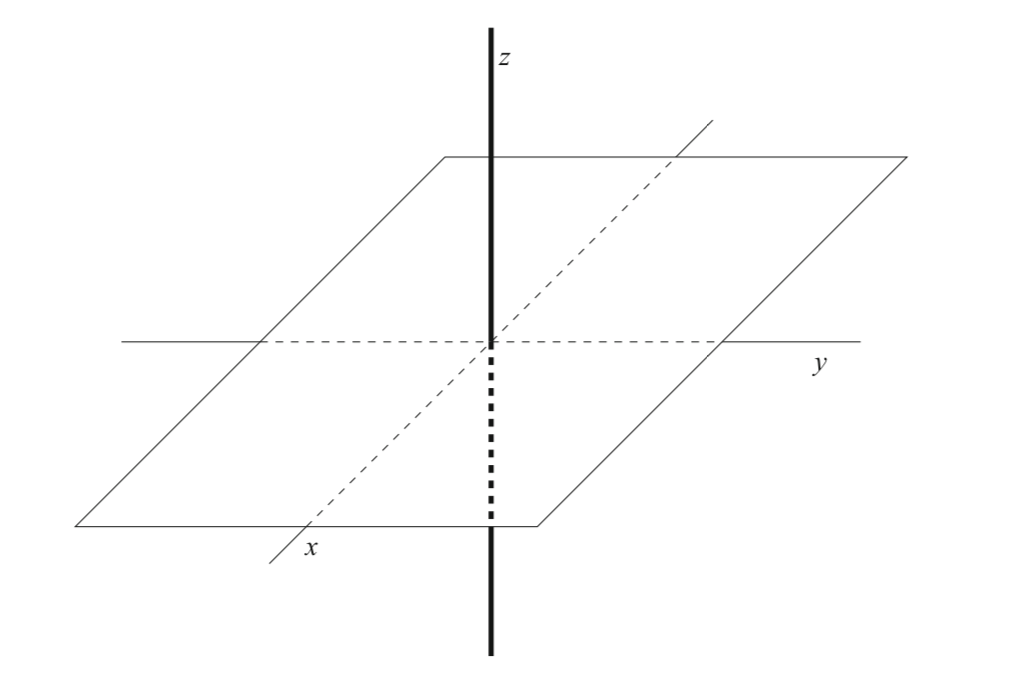
\includegraphics[width=1.0\textwidth]{affineVariety.png}
 	\caption[Example of an affine variety]{Affine variety defined by $(xz,yz)$. Image source: (\cite{algGeom}, page $9$).}
 	\label{fig1}
 \end{figure}

 \begin{DF}
Let $R$ be a commutative ring, then any non-empty subset $I \subseteq R$ is called a (two-sided) \textbf{ideal} of $R$ if it satisfies following requirements:
\begin{itemize}
\item $I \neq \emptyset,$\hfill ($I$ is a non-empty set)
\item $\forall f,g \in I: (f + g) \in I,$ \hfill ($I$ is closed under addition)
\item $\forall f \in I,\ \forall h \in R: hf \in I.$ \hfill ($I$ is closed under multiplication by $R$)
\end{itemize}
\end{DF}
\noindent In this thesis we are mostly concerned about ideals generated by a finite number of polynomials over some field.
\begin{DF}
Let $X = (x_1, \ldots ,x_n)$ be an ordered $n$-tuple of formal variables and let $f_1,\ldots,f_s \in \mathbb{F}[X] $ be an $s$-tuple of polynomials. Then we set
$$
\langle f_1, \ldots, f_x \rangle := \{ \sum_{i=1}^n h_if_i\ |\ h_1,\ldots,h_s \in \mathbb{F}[X]\}
$$
\end{DF}
\noindent to be the \textbf{ideal generated by} polynomials $f_1,\ldots,f_s$.
\begin{RM}
Every ideal $I$ of $\mathbb{F}[X]$ is finitely generated, which means:
$$
\exists s \in \mathbb{N},\ \exists f_1,\ldots,f_s \in \mathbb{F}[X]: I = \langle f_1, \ldots, f_s \rangle,
$$
\noindent and we say that the polynomials $f_1,\ldots,f_s$ form a \textbf{basis} of $I$. Note that a given ideal $I$ may have many different bases. If we have two different bases $B_1 = (f_1,\ldots,f_s),\ s \in \mathbb{N},$ and $B_2 = (g_1, \ldots, g_t),\ t \in \mathbb{N},$ of the same ideal $I$ in $\mathbb{F}[X]$, such that $I = \langle B_1\rangle = \langle B_2 \rangle,$ then the affine varieties ${\text{in }\mathbb{F}^n}$, defined by the bases $B_1$ and $B_2$, are the same.
$$
\mathcal{V}(B_1) = \mathcal{V}(B_2).
$$
\end{RM}
\begin{DF}
Let $\mathcal{V} \subseteq \mathbb{F}^n$ be an affine variety and let $X = (x_1, \ldots ,x_n)$ be an ordered $n$-tuple of formal variables. Then we set 
$$
\mathbf{I}(\mathcal{V}) := \{ f \in \mathbb{F}[X]\ |\ \forall a \in \mathcal{V}: f(a) = 0\}.
$$
\noindent to be the \textbf{ideal of affine variety} $\mathcal{V}$.
\end{DF}
\begin{RM}
The natural question to ask is whether $\mathbf{I}(\mathcal{V}(f_1,\ldots,f_s)) = \langle f_1,\ldots,f_s \rangle.$ The answer, unfortunately, is not always yes, but the following set inclusion holds:
$$
\langle f_1,\ldots,f_s \rangle \subseteq \mathbf{I}(\mathcal{V}(f_1,\ldots,f_s)) .
$$
\end{RM} 
\begin{DF}
Let $f,g \in \mathbb{F}[x]$ be two non-constant polynomials of degrees $l,m \in \mathbb{Z}_{>0}$, deg$(f) = l,\ $deg$(g)=m$. Then $f,g$ have a common factor in $\mathbb{F}[x]$ if and only if there are polynomials $A,B \in \mathbb{F}[x]$, such that:
\begin{enumerate}
\item $A \neq 0,\ B \neq 0,$ 
\item deg$(A) \leq m - 1,$ deg$(B) \leq l - 1,$
\item $Af  + Bg = 0.$
\end{enumerate}
\noindent To decide whether polynomials $f,g$ have a common factor, we can rewrite $Af  + Bg = 0$ as a system of linear equations and find a non-zero solution.
\begin{align*}
A &= u_0x^{m-1} + \cdots + u_{m-1}, \\
B &= v_0x^{l-1} + \cdots + v_{l-1}, \\
f &= c_0x^l + \cdots + c_l, \quad c_0 \neq 0, \\
g &= d_0x^m + \cdots + d_m, \quad d_0 \neq 0. \\
\end{align*}
If we compare the coefficients of powers of $x$, then we get a system of linear equations with variables $u_i,\ i \in \{0,1,\ldots	, m - 1\}$ and $v_j,\ j \in \{0,1,\ldots, l - 1\}$ and coefficients $c_i, d_j \in \mathbb{F}.$ The coefficient matrix of this system is called the \textbf{Sylvester matrix} of $f$ and $g$ with respect to $x$, denoted by Syl$_{x}(f,g)$. Syl$_{x}(f,g)$ is the following $(l + m) \times (l + m)$ matrix:
$$
\text{Syl}_{x}(f,g) := \begin{pmatrix}
c_0 &  &  &  &             d_0 &  &  &  \\
c_1 & c_0 &  &  &        d_1 & d_0 &   &  \\
c_2 & c_1 & \ddots &  & d_2 & d_1 & \ddots  &  \\
\vdots & & \ddots & c_0 & \vdots &  & \ddots & d_0 \\
 &  \vdots &  & c_1 &  & \vdots &  & d_1 \\
c_l &  &  &  &  d_m&  &  & \\
 & c_l &  & \vdots &  & d_m &  & \vdots \\
 &  & \ddots &  &  &  & \ddots &  \\
\coolunder{m \text{ columns}}{\hphantom{..} & \hphantom{...} & \hphantom{..}  & c_l & }\coolunder{l \text{ columns}}{\hphantom{...} & \hphantom{...} & \hphantom{......} & d_m \hphantom{..}} \\
\end{pmatrix},
$$ \\  \\
\noindent where the empty spaces are filled by zeros. \\ \\
\noindent The determinant (we expect our reader is familiar with this term, if not, you can find its definition in any decent linear algebra textbook) of the Sylvester matrix is called the \textbf{resultant} of polynomials $f$ and $g$ with respect to $x$, and is denoted by Res$_{x}(f,g)$. Furthermore, $f,g$ have a common factor in $\mathbb{F}[x]$ if and only if Res$_x(f,g) = 0$, which is equivalent to the above-presented system of linear equations having a non-zero solution. An example of the resultant of two quadratic polynomials is shown on page \pageref{resExample}. 
\\ \\
\noindent If $f,g$ have a common factor $h \in \mathbb{F}[x],\ \text{deg}(h) \geq 1$, then there exist ${f_1, g_1 \in \mathbb{F}[x]}$, such that:
$$
f = hf_1, \quad g = hg_1.
$$
\end{DF}
\noindent Moreover, if $\mathbb{F}$ is an algebraically closed field, polynomials $f,g$ have a common root $r \in \mathbb{F}$. Since $\mathbb{F}$ is algebraically closed field, a (non-constant) common factor $h$ has a root ${r \in \mathbb{F}}$: ${h(r) = 0}$. Therefore, $r$ is a common root of polynomials $f,g$:
\begin{align*}
(hf_1)(r) &= h(r)f_1(r) = 0f_1(r) = 0 \Leftrightarrow f(r) = 0 ,\\
(hg_1)(r) &= h(r)g_1(r) = 0g_1(r) = 0 \Leftrightarrow g(r) = 0.\\
\end{align*}

\subsection{Monomial Ordering}
\noindent The notion of ordering of terms in a polynomial is a key ingredient in many algorithms, e.g. the long division of polynomials. When dealing with polynomials in only one variable, we usually write the terms of the polynomial in the decreasing order by their monomial degree. \\
\noindent For example, ${f(x) = 2x^4 - 10x^3 + x^2 + x -12}$. The degree ordering on the one-variable monomials is straightforward:
$$
\cdots > x^{m+1} > x^m > x^{m-1} \cdots > x^2 > x > 1
$$
We would like to establish an ordering on the terms in polynomials in $\mathbb{F}[X],$ where $X = (x_1, \ldots, x_n)$. First, we note that we can reconstruct the monomial $X^{\alpha} = x_1^{\alpha_1}\cdots x_n^{\alpha_n}$ from the $n$-tuple of exponents $\alpha = (\alpha_1,\ldots, \alpha_n) \in \mathbb{Z}_{\geq 0}^n.$ Based on this observation, we define an ordering $>$ on the space $\mathbb{Z}_{\geq 0}^n$ which also gives us an ordering on the monomials $\in \mathbb{F}[X].$ If for some $\alpha, \beta \in  \mathbb{Z}_{\geq 0}^n$ and some ordering $>$ holds: $\alpha > \beta$ we also say that $X^\alpha > X^\beta.$ In this thesis, we only consider \textbf{total orderings}, which means that for every pair of monomials $X^\alpha$ and $X^\beta$, exactly one of the three statements holds:
\begin{itemize}
\item $X^\alpha > X^\beta,$\hfill (when $\alpha > \beta$)
\item $X^\alpha = X^\beta,$\hfill (when $\alpha = \beta$)
\item $X^\alpha < X^\beta,$\hfill (when $\alpha < \beta$)
\end{itemize}
\noindent and $>$ is transitive:
$$
\forall \alpha, \beta, \gamma \in \mathbb{Z}_{\geq 0}^n: (X^\alpha > X^\beta \land X^\beta > X^\gamma) \implies X^\alpha > X^\gamma.
$$
\noindent We also require that multiplication of two polynomials does not change the relative order of terms. Therefore, the following property for $>$ must hold:
$$
\forall \alpha, \beta, \gamma \in \mathbb{Z}_{\geq 0}^n: X^\alpha > X^\beta \implies X^\alpha X^\gamma > X^\beta X^\gamma.
$$
\noindent Which in terms of the exponent vectors means: 
$$
\forall \alpha, \beta, \gamma \in \mathbb{Z}_{\geq 0}^n: \alpha > \beta \implies \alpha + \gamma > \beta + \gamma.
$$
\noindent To summarize all the requirements, we make the following definition.
\begin{DF}
A \textbf{monomial ordering} $>$ on $\mathbb{F}[X]$, where $X = (x_1, \ldots, x_n)$ is a relation $>$ on $\mathbb{Z}_{\geq 0}^n$ satisfying:
\begin{itemize}
\item $>$ is a total order on $\mathbb{Z}_{\geq 0}^n$,
\item $\forall \alpha, \beta, \gamma \in \mathbb{Z}_{\geq 0}^n: \alpha > \beta \implies \alpha + \gamma > \beta + \gamma,$
\item $\forall A \subseteq \mathbb{Z}_{\geq 0}^n,\ A \neq \emptyset: \exists \alpha \in A,\ \forall \beta \in A \setminus \{\alpha \}: \beta > \alpha.$ 
\end{itemize}
\noindent The last requirement tells us, that in every non-empty subset of $\mathbb{Z}_{\geq 0}^n$ there exists a minimum element under the relation $>$.
\end{DF}
\begin{DF}
Let $\alpha = (\alpha_1, \ldots, \alpha_n),\ \beta = (\beta_1, \ldots, \beta_n)\in \mathbb{Z}_{\geq 0}^n.$ \textbf{Lexicographic Order} (\textbf{lex}), denoted by $>_{lex}$, is a generalisation of the way words are ordered in a dictionary. We say $\alpha >_{lex} \beta$ if the leftmost non-zero entry of the vector difference $\alpha - \beta \in \mathbb{Z}^n$ is positive. We write: $X^\alpha >_{lex} X^\beta$ if $\alpha >_{lex} \beta$.
\end{DF}
For example:
\begin{itemize}
\item $(10,4,3) >_{lex} (10, 3, 4),$ since $\alpha - \beta = (0,1,-1)$.
\item $(7,5,3,1) >_{lex} (7, 5, 2, 4),$ since $\alpha - \beta = (0,0,1,-3)$.
\item The variables $x_1,\ldots,x_n$ are ordered in the usual way by the lexicographic order:
$$
(1,0,\ldots,0) >_{lex} (0,1,0,\ldots, 0) >_{lex} \cdots >_{lex} (0, \ldots, 0, 1),
$$
so $x_1 >_{lex} x_2 >_{lex} \cdots >_{lex} x_n.$ \\ \\
In the rest of this thesis, we assume $x >_{lex} y >_{lex} z,$ unless stated otherwise.
\end{itemize} 
\begin{DF}
Let $\alpha = (\alpha_1, \ldots, \alpha_n),\ \beta = (\beta_1, \ldots, \beta_n)\in \mathbb{Z}_{\geq 0}^n.$ \textbf{Graded Lexicographic Order} (\textbf{grlex}), denoted by $>_{grlex}$, at first orders the terms by the total degree, then break ties using the standard lexicographic order defined above. 
$$
\alpha >_{grlex} \beta: (|\alpha| > |\beta|) \lor (|\alpha| = |\beta| \land \alpha >_{lex} \beta),
$$
where $|\alpha| = \sum_{i=1}^n \alpha_i$ and $|\beta| = \sum_{i=1}^n \beta_i$.
\end{DF}
\begin{itemize}
\item $(10,2,6) >_{grlex} (10, 3,4),$ since $|\alpha| = 18 > |\beta| = 17$.
\item $(7,5,3,1) >_{grlex} (7, 5, 2, 4),$ since $|\alpha| = 16 = |\beta|$ and $\alpha >_{lex} \beta$.
\item The variables $x_1,\ldots,x_n$ are ordered in the same way as by $>_{lex}$ order:
$$
(1,0,\ldots,0) >_{grlex} (0,1,0,\ldots, 0) >_{grlex} \cdots >_{grlex} (0, \ldots, 0, 1),
$$
\end{itemize} 
\begin{DF}
Let $\alpha = (\alpha_1, \ldots, \alpha_n),\ \beta = (\beta_1, \ldots, \beta_n)\in \mathbb{Z}_{\geq 0}^n.$ \textbf{Graded Reverse Lexicographic Order} (\textbf{grevlex}), denoted by $>_{grevlex}$, is somehow less intuitive order, but it is usually the most efficient for computations.  We say $\alpha >_{grevlex} \beta$ if $|\alpha| > |\beta|$ or if $|\alpha| = |\beta|$ and the rightmost non-zero entry of vector difference $\alpha - \beta \in \mathbb{Z}^n$ is negative.
\end{DF}
\begin{itemize}
\item $(4,7,1) >_{grevlex} (4, 2,5),$ since $|\alpha| = 12 > |\beta| = 11$.
\item $  (7, 5, 1, 3) >_{grevlex} (1,5,3,7),$ since $|\alpha| = 16 = |\beta|$, \\
and $\alpha - \beta = (6,0,-2, -4),\ -4 < 0$.
\item The variables $x_1,\ldots,x_n$ are ordered in the same way as by $>_{lex}$ order:
$$
(1,0,\ldots,0) >_{grevlex} (0,1,0,\ldots, 0) >_{grevlex} \cdots >_{grevlex} (0, \ldots, 0, 1),
$$
\end{itemize}
Now we show, how would the polynomial $f(x,y,z) = 4xy^2z + 4z^2 - 5x^3 + 7x^2z^2 \in \mathbb{Z}[x,y,z]$ be written, if we reorder its terms by a monomial order in decreasing order:
\begin{itemize}
\item With respect to the lex order:
$$
f(x,y,z) = -5x^3 + 7x^2z^2 + 4xy^2z + 4z^2.
$$
\item With respect to the grlex order:
$$
f(x,y,z) = 7x^2z^2  + 4xy^2z -5x^3 + 4z^2.
$$
\item With respect to the grevlex order:
$$
f(x,y,z) = 4xy^2z + 7x^2z^2  -5x^3 + 4z^2.
$$
The first two terms have the same total degree of $4$ and $xy^2z >_{grevlex} x^2z^2$ because $(1,2,1) - (2,0,2) = (-1,2,-1)$ and $-1 < 0$.
\end{itemize} 
\begin{DF}
Let $f = \sum_\alpha a_\alpha X^\alpha$ be a non-zero polynomial in $\mathbb{F}[X]$, and let $>$ be a monomial order.
\begin{itemize}
\item The \textbf{multidegree} of $f$ is:
$$
\text{multideg}(f) := \text{max}(\alpha \in \mathbb{Z}_{\geq 0}^n\ |\ a_\alpha \neq 0),
$$
the maximum is taken with respect to $>$.\\ \\
Let $g \in \mathbb{F}[X],\ g \neq 0$, then multideg$(fg) = \text{multideg}(f) + \text{multideg}(g)$. If $(f + g) \neq 0$, then $\text{multideg}(f + g) \leq \text{max}(\text{multideg}(f),\ \text{multideg}(g))$, more precisely if the multidegrees of $f$ and $g$ are not equal, then the equality occurs: $\text{multideg}(f + g) = \text{max}(\text{multideg}(f),\ \text{multideg}(g))$.
\item The \textbf{leading coefficient} of $f$ is:
$$
\text{LC}(f) := a_{\text{multideg}(f)} \in \mathbb{F}.
$$
\item The \textbf{leading monomial} of $f$ is:
$$
\text{LM}(f) := X^{\text{multideg}(f)} \in \mathbb{F}[X],
$$
with coefficient $1$.
\item The \textbf{leading term} of $f$ is:
$$
\text{LT}(f) := (\text{LC}(f)\cdot \text{LM}(f)) \in \mathbb{F}[X].
$$
\end{itemize}
\end{DF}
\noindent To illustrate that, let $f(x,y,z) = 4xy^2z + 4z^2 - 5x^3 + 7x^2z^2 \in \mathbb{Z}[x,y,z]$ as before and let's use $>_{grevlex}$ order.
\begin{align*}
f(x,y,z) &= 4xy^2z + 7x^2z^2  -5x^3 + 4z^2, \text{ (in  grevlex order)}\\
\text{multideg}(f)&=(1,2,1), \\
\text{LC}(f)&=4, \\
\text{LM}(f)&=xy^2z, \\
\text{LT}(f)&=4xy^2z. \\
\end{align*}
Now we can formulate the idea of a general division algorithm in $\mathbb{F}[X]$.
\begin{RM}
Let $p, q \in \mathbb{F}[X]$ be two monomials, we say the monomial $p$ is \textbf{divisible} by the monomial $q$ if and only if there exists a monomial $h \in \mathbb{F}[X]$, such that: $p = qh$. We denote it by $q\ |\ p$ which we read  as \textbf{$\mathbf{q}$ divides $\mathbf{p}$}.
\end{RM}
\begin{DF}
Let $>$ be a monomial order on $\mathbb{Z}_{\geq 0}^n$, let $F = (f_1, \ldots, f_s)$ be an ordered $s$-tuple of polynomials in $\mathbb{F}[X],$ where $X = (x_1, \ldots, x_n)$. Then every $f \in \mathbb{F}[X]$ can be written as:
$$
f = q_1f_1 + \cdots + q_sf_s + r,
$$
where $q_i, r \in \mathbb{F}[X]$, and either $r = 0$ (is a zero polynomial) or $r$ is a linear combination, with coefficients in $\mathbb{F}$, of monomials $\in \mathbb{F}[X]$, none of those monomials is divisible by any of LT$(f_1), \ldots,$LT($f_s$).
We call polynomial $r$ a \textbf{remainder} of $f$ on division by $F$. Furthermore, if $q_if_i \neq 0$, then
$$
\text{multideg}(f) \geq \text{multideg}(q_if_i).
$$
\end{DF}
\noindent We won't describe the division algorithm itself in this thesis. If you are not familiar with this algorithm, please refer to~\cite{algGeom} on pages 61-68, where the algorithm is discussed in great detail.\\ \\
\noindent Unfortunately, the remainder is not uniquely characterised and depends on the order of the divisors in the set $F$, and also on the monomial order itself. \\ \\
\noindent Furthermore, we would like to use this idea to answer the ideal membership problem. Let $f, f_1, \ldots, f_s \in \mathbb{F}[X]$ and let $I = \langle f_1, \ldots, f_s \rangle$ be an ideal. We would like to determine whether $f \in I$ is true. We can clearly state, that if the remainder $r$ obtained after division of $f$ by $F = (f_1, \ldots, f_s)$ is $0$, then $f$ has to be an element of the ideal $I$. So $r=0$ is a sufficient condition for the ideal membership. However, it isn't a necessary condition for $f$ being in the ideal. To remedy this situation, we try to describe a \textquote{good} basis of the ideal $I$, such that the remainder $r$ on division by the polynomials of this basis is uniquely determined, and that the condition $r=0$ is equivalent to the membership in the ideal. Exactly those good properties have Gröbner bases, which we describe in the following section.
\section{Gröbner Bases}
Gröbner bases may be used to solve many problems about polynomial ideals in an algorithmic or computational fashion. It is one of the most used methods for solving systems of multivariate polynomial equations, i.e. calculating the affine variety defined by those polynomial equations. This section is based on~\cite{algGeom}.
\begin{DF}
An ideal $I \subseteq \mathbb{F}[X]$ is called a \textbf{monomial ideal} if there exists a (possibly infinite) subset $A \subseteq \mathbb{Z}_{\geq 0}^n$, such that $I$ consists of all polynomials which are finite sums: $\sum_{\alpha \in A} h_\alpha X^\alpha$, where $h_\alpha \in \mathbb{F}[X].$ We can then write $I$ in the form: $I = \langle X^\alpha \ |\ \alpha \in A\rangle.$ Monomial $X^\beta, \beta \in \mathbb{Z}_{\geq 0}^n,$ lies in the ideal $I$ if and only if there exist $\alpha \in A$, such that $X^\alpha \ |\ X^\beta$ ($X^\beta$ is divisible by some $X^\alpha$). 
\end{DF}
\begin{RM}
\textbf{(Dickson's Lemma).} Any monomial ideal ${I = \langle X^\alpha \ |\ \alpha \in A\rangle \subseteq \mathbb{F}[X]}$ can be written in the form $I = \langle X^{\alpha(1)}, \ldots, X^{\alpha(s)}\rangle,\ s \in \mathbb{N},$ where $\alpha(1), \ldots, \alpha(s)$\\ $\in A$. In particular, $I$ has a finite basis $(X^{\alpha(1)}, \ldots, X^{\alpha(s)})$.
\end{RM}
\begin{DF}
A monomial ideal $I \subseteq \mathbb{F}[X]$ has a finite basis $(X^{\alpha(1)}, \ldots, $\\$X^{\alpha(s)})$ with the property that $X^{\alpha(i)}$ does not divide $X^{\alpha(j)}$ for any $i \neq j$. Furthermore, this basis is unique and is called the \textbf{minimal basis} of $I$.
\end{DF}
\begin{DF}
Let $I \subseteq \mathbb{F}[X],\ I \neq {0},$ be an ideal and fix a monomial order on $\mathbb{F}[X]$.  Then:
\begin{itemize}
\item We denote by LT$(I)$ the \textbf{set of leading terms} of non-zero elements of~$I$.
$$
\text{LT}(I) = \{ cX^\alpha \ |\ \exists f \in I \setminus \{0\}: \text{LT}(f)= cX^\alpha \}.
$$
\item We denote by $\langle \text{LT}(I) \rangle$ the \textbf{ideal of leading terms} of $I$. $\langle \text{LT}(I) \rangle$ is a monomial ideal, therefore there exist a finite set $g_1,\ldots, g_t \in I,\ t \in \mathbb{N},$ such that:
$$
\langle \text{LT}(I) \rangle = \langle \text{LT}(g_1), \ldots, \text{LT}(g_t) \rangle.
$$
\end{itemize}
\end{DF}
\begin{DF}
Fix a monomial order on $\mathbb{F}[X]$, therefore every polynomial $f \in \mathbb{F}[X]$ has a unique leading term. A finite subset $G = \{g_1, \ldots, g_t \}$ of an ideal $I \subseteq \mathbb{F}[X],\ I \neq \{ 0 \}$ is said to be a \textbf{Gröbner basis} (or \textbf{standard basis}) if:
$$
\langle \text{LT}(g_1), \ldots, \text{LT}(g_t) \rangle = \langle \text{LT}(I) \rangle.
$$
Additionally, we define the Gröbner basis of the zero ideal $\{0\}$ to be the empty set $\emptyset$ using the convention that $\langle \emptyset \rangle = \{0\}.$
\end{DF}
\begin{RM}
Every ideal $I \subseteq \mathbb{F}[X]$ has a Gröbner basis. Furthermore, any Gröbner basis for an ideal $I$ is a basis of $I$. Gröbner bases for ideals in polynomial rings were introduced by B. Buchberger in his PhD thesis (1965)~\cite{bruno} and named by him in honour of his thesis's advisor W. Gröbner. Buchberger also developed fundamental algorithms to find and work with Gröbner bases. In many computer algebra systems, there is usually used an alternative spelling \textquote{Groebner bases}.
\end{RM}
\phantom{.}
\phantom{.}
\noindent Now we will mention few important properties of Gröbner bases.
\begin{RM}
Let $I \subseteq \mathbb{F}[X]$ be an ideal and let $G = \{g_1, \ldots, g_t\}$ be a Gröbner basis of $I$. Then for any $f \mathbb{F}[X],$ there is a unique polynomial $r$ with those two properties:
\begin{itemize}
\item No term of $r$ is divisible by any of LT$(g_1),\ldots,$LT$(g_t)$.
\item $\exists g \in I:\ f = g + r.$
In particular, $r$ is the remainder on division of $f$ by set $G$ no matter, how are the elements of $G$ listed, when using the division algorithm. 
\end{itemize}
Polynomial $r$ is called the \textbf{normal form} of f. \\ \\ 
\noindent Polynomial $f \in I$ if and only if the remainder $r$ on division $f$ by $G$ is zero, $r = 0.$
\end{RM}
\begin{DF}
Let $f \in \mathbb{F}[X]$ be a polynomial and let $F = (f_1, \ldots, f_s) \subseteq \mathbb{F}[X]$ be an ordered $s$-tuple of polynomials. We will denote the remainder on the division of $f$ by $F$ by $\overline{f}^F$. If $F$ is a Gröbner basis for $\langle f_1, \ldots, f_s \rangle$, then we can regard $F$ as a set without any particular order, because the remainder on the division by a Gröbner basis is unique.
\end{DF}
\begin{DF}
Let $f,g \in \mathbb{F}[x_1,\ldots,x_n]$ be non-zero polynomials. Let $\alpha = \text{multideg}(f)$ and $\beta = \text{multideg}(g)$, then ${\gamma = (\gamma_1,\ldots,\gamma_n)},$ where ${\gamma_i = \text{max}(\alpha_i,\beta_i)}$ for each $i \in \{1,\ldots,n\}.$ We call $X^\gamma$ the \textbf{least common multiple} of LM$(f)$ and LM$(g)$, denoted by $X^\gamma = \text{lcm(LM}(f),(\text{LM}(g)).$ \\ \\
\noindent The \textbf{S-polynomial} of $f$ and $g$ is the combination:
$$
\text{S}(f,g) := \frac{X^\gamma}{\text{LT}(f)}\cdot f - \frac{X^\gamma}{\text{LT}(g)}\cdot g.
$$
\end{DF}
\noindent For example, let $f=x^3y^2 - x^2y^3 + x$ and $g = 3x^4y + y^2$ in $\mathbb{R}[x,y]$ with grlex order. Then $\gamma = (4,2)$ and
\begin{align*}
\text{S}(f,g) &= \frac{x^4y^2}{x^3y^2}\cdot f - \frac{x^4y^2}{3x^4y}\cdot g \\
&= x\cdot f - \frac{1}{3}y^3\cdot g \\
&= -x^3y^3 + x^2 - \frac{1}{3}y^3.
\end{align*}
An S-polynomial is \textquote{designed} to produce cancellation of the leading terms.
\begin{DF}
\textbf{(Buchberger's Criterion)}: Let $I$ be a polynomial ideal. Then a basis $G = \{g_1,\ldots,g_t\}$ of $I$ is a Gröbner basis of $I$ if and only if for all pairs $i\neq j$, the remainder on division by S$(g_i,g_j)$ by $G$ (listed in some order) is zero.
\end{DF}
\noindent Based on this criterion, there is the Buchberger's algorithm (described on page 91 in~\cite{algGeom}), that computes the Gröbner basis.
\begin{DF}
A \textbf{reduced Gröbner basis} for a polynomial ideal $I$ is a Gröbner basis $G$ for $I$ such that:
\begin{itemize}
\item $\forall p \in G: \text{LC}(p) = 1.$
\item $\forall p \in G$: no monomial $p$ lies in $\langle\text{LT}(G \setminus \{p\}) \rangle.$
\end{itemize}
\end{DF}
\noindent Any polynomial ideal $I\neq \{\emptyset\}$ for a given monomial order has a unique reduced Gröbner basis. 
\\
\\
\noindent Now we describe, how to use Gröbner bases for finding all the solutions of a system of multivariate polynomial equations.
\begin{DF}
Given ideal $I = \langle f_1,\ldots,f_s\rangle \subseteq \mathbb{F}[x_1,\ldots,x_n]$, the $l$-th \textbf{elimination ideal} $I_l$ is the ideal of $\mathbb{F}[x_{l+1},\ldots,x_n]$ defined by:
$$
I_l := I \cap \mathbb{F}[x_{l+1},\ldots,x_n].
$$
\end{DF}
\noindent Note that different orderings of the variables lead to different elimination ideals.
\begin{DF}
\textbf{(The Elimination Theorem).} Let $I \subseteq \mathbb{F}[x_1,\ldots,x_n]$ be an ideal and let $G$ be a Gröbner basis of $I$ with respect to lex order where $x_1 > x_2 > \cdots > x_n$. Then, for every $0\leq l \leq n$, the set:
$$
G_l := G \cap \mathbb{F}[x_{l+1},\ldots,x_n]
$$
is a Gröbner basis of the $l$-th elimination ideal $I_l$.
\end{DF}
\vphantom{.}
\noindent To find all the points in the affine variety $\mathcal{V}(I)$, we build up the solutions one coordinate at a time. At first, we find the affine variety $\mathcal{V}(I_{n-1})$, which is equivalent to finding the roots of a univariate polynomial in $\mathbb{F}[x_n]$. We call any solution $(a_n) \in \mathcal{V}(I_{n-1})$ a \textbf{partial solution} of the original system of equations. Next step is to extend a partial solution $(a_n)$ to a partial solution $(a_{n-1},a_n) \in \mathcal{V}(I_{n-2})$. To do that, we substitute $(a_n)$ into all the polynomial equations in $I_{n-2}$. Thereafter, we obtain a univariate polynomial equation in $\mathbb{F}[x_{n-1}]$, which we can conveniently solve. Note that not every partial solution in $\mathcal{V}(I_{n-1})$ extends to a partial solution in $\mathcal{V}(I_{n-2})$. We repeat this process until we find $\mathcal{V}(I_0) = \mathcal{V}(I)$, a set of all \textbf{complete solutions} to the original system of equations.
\begin{DF}
\label{triagForm}
Let $G = \{g_1,\ldots,g_s\}$ be the reduced Gröbner basis for a zero-dimensional ideal $I \subset \mathbb{F}[X_1,\ldots,X_n]$ with respect to the lexicographic order of monomials with $X_1 >_{\text{lex}} \cdots >_{\text{lex}} X_n$ and ordered so that every LT$(g_j) >_{\text{lex}} $LT($g_{j+1}$). Then for each $i \in \{1,\ldots,n\}$ there is some $j=j(i)$ for which LT$(g_j)=x_i^{d_i}$ for some $d_i > 0.$ This is called the \textbf{triangular form} and is especially convenient for finding all the points, that lie in the affine variety defined by the polynomials $g_1,\ldots,g_n$. The last polynomial in $G$ is univariate: $g_s = g_s(X_n)$. We can find its roots (a partial solution) and substitute them into all the other polynomials in $G$. After such substitution, at least one of the earlier polynomials $g_i,\ i \in \{1,\ldots,s-1\}$ is univariate in $X_{n-1}$. We can repeat this process until we find the affine variety $\mathcal{V}(G)$, the set of all complete solutions. This method is called \textbf{backsolving} or \textbf{backsubstitution}, for more information see~\cite{week11}.
\end{DF}

\chapter{Elliptic Curves and the Discrete Logarithm Problem}
In this chapter, we revise the theory of elliptic curves and state the elliptic curve discrete logarithm problem (ECDLP). In the last section, we also introduce the reader to the concept of summation polynomials, which are the primary building block in many specialised algorithms (exploiting the particular group structure) solving the ECDLP. Examples of such algorithms are discussed in detail in chapter \ref{specAlg}.
\section{Elliptic Curves}
This section focuses on elliptic curves over finite fields and groups of points on them. At first, we define what is a general elliptic curve. Afterwards, we show how to define an Abelian group on the set of points of an elliptic curve. This section is based mostly on~\cite{mky}.
\begin{DF}
An \textbf{elliptic curve} over a (prime order) finite field $GF(p),$ \\ $p > 3,\ p$ prime, defined by the short Weierstrass equation, is a set:
$$
E(GF(p)) := \{(x,y)\ |\ x,y \in \mathbb{F},\ y^2 = x^3 + Ax+B\} \cup \{ \mathcal{O} \},
$$
where $A, B \in GF(p)$ are \textbf{coefficients of the elliptic curve}. Coefficients $A,B$ have to satisfy the following condition: $4A^3 + 27B^2 \neq 0$, which guarantees the right-hand side polynomial $f(x)=x^3 + Ax+B$ has 3 distinct roots. Elliptic curves are \textbf{non-singular} curves, i.e. they don't have any cusps nor self-intersections. \\
\noindent Point $\mathcal{O}$ is called the \textbf{point at infinity} (in the projective plane).
\end{DF}
\begin{DF}
Let $E(GF(p))$ be an elliptic curve, and let $P,Q \in E(GF(p)),$\\${P=(x_1,y_1),\ Q=(x_2,y_2)}$ be two points on the elliptic curve $E$. We define the binary operation $\oplus: E(GF(p)) \times E(GF(p)) \to E(GF(p))$, called \textbf{addition on the elliptic curve} $E(GF(p))$, as follows:
\begin{itemize}
\item Point at infinity $\mathcal{O}$ is an identity element of the operation $\oplus$, therefore if $P = \mathcal{O},\ P \oplus Q = Q,$ or if $Q = \mathcal{O},\ P \oplus Q = P.$
\item Else if $x_1 = x_2$ and $P\neq Q$, $P\oplus Q = \mathcal{O}.$ Point at infinity $\mathcal{O}$ is the identity element of the operation $\oplus$. Therefore, point $Q$ is the \textbf{additive inverse} of the point $P$, denoted by $\ominus P$. We now state the explicit formula for the point $\ominus P$, we know its $x$-coordinate is $x_1$, and we use the $E$ equation and substitute $X$ with $x_1$:
$$
Y^2  = (x_1^3 + Ax_1 + B),
$$
which is a quadratic equation in the variable $Y$. We already know one of its roots $y_1$, the other root has to be $-y_1$. Therefore:
$$\ominus P = (x_1, -y_1).$$
\item Else if $x_1 \neq x_2$, let $\lambda$ be the slope of the line defined by the points $P,Q.$
$$
\lambda = \frac{y_2 - y_1}{x_2 - x_1},
$$
Else if $P = Q$ (\textbf{point doubling}), let $\lambda$ be the slope of the tangent line to the elliptic curve equation at the point $P.$
$$
\lambda = \mathlarger{\mathlarger{\frac{\frac{\mathrm{d}E}{\mathrm{d}X}}{\frac{\mathrm{d}E}{\mathrm{d}Y}}}}(x_1, y_1) = \frac{3x_1^2+ A}{2y_1}, 
$$
where $\mathrm{d}E/\mathrm{d}X$ and  $\mathrm{d}E/\mathrm{d}Y$ are the derivatives of the elliptic curve equation with respect to $X,Y$. \\ \\
\noindent The result of the operation $\oplus$ is:
\begin{align*}
x_3 &= \lambda^2 - x_1 - x_2, \\
y_3 &= \lambda(x_1 - x_3) - y_1, \\ 
 P \oplus Q &= (x_3, y_3).
\end{align*}
\end{itemize}
\end{DF}
\begin{DF}
A set of points on the elliptic curve defined by the short Weierstrass equation and the binary operation $\oplus$ form an Abelian group, $(E(GF(p)), \oplus)$ is a group, and we denote it by $E(p)$. If we want to explicitly mention the coefficients $A,B$ we use $E_{A,B}(p)$.
\end{DF}
\begin{NRM}
Let $P \in E(p)$ be a point on an elliptic curve $E$ over $GF(p)$. To shorten the notation of the repeated application of the group law, we use the notation introduced in chapter 1. To remind our readers; \textbf{multiplication} of a point on the elliptic curve $E$ by an integer $t$ has the following meaning:
$$
\forall P \in E(p),\ \forall t \in \mathbb{Z}: tP := \begin{cases} \underbrace{P \oplus P \oplus \cdots \oplus P}_{\text{$t$-times}} &\quad t > 0, \\
\mathcal{O} \text{ (identity element) } &\quad t = 0, \\
\underbrace{(\ominus P) \oplus (\ominus P) \oplus \cdots \oplus (\ominus P)}_{\text{$t$-times}} &\quad t < 0.
\end{cases}
$$
\end{NRM}
\begin{DF}\textbf{(Hasse's Theorem.)} \label{hase}Let $E$ be an elliptic curve over a finite field $GF(p),\ p$ prime. Then the following inequalities hold:
$$
p + 1 -2\sqrt{p} \leq \#E(p) \leq p + 1 + 2\sqrt{p}.
$$
In other words, the number of points in the elliptic curve group $E(p)$ is close to the prime $p$. To calculate the exact number of points in $E(p)$, the Schoof-Elkies-Atkin's (SEA) algorithm is commonly used. The time complexity of the SEA algorithm amounts to $O(\log^{2\mu + 2}(p))$ bit operations, where $\mu$ is a constant such that two $T$-bit integers can be multiplied in time $T^\mu$, and the space complexity is $O(\log^2(p)).$ The detailed description of the SEA algorithm can be found in chapter 17 of~\cite{handbook}. 
\end{DF}
\subsection{Complexity of Arithmetic Operations on an Elliptic Curve} 
The complexity of arithmetic operations on $E$ is based on the complexity of operations in the underlying finite field $GF(p)$. The exact number of arithmetic operations depends on the used algorithm, its implementation, and on the architecture of the CPU, where the particular code is executed. Table \ref{tblComp} provides a brief summary of the relationship between the operations on elliptic curve $E$ and the number of arithmetic operations in the underlying finite field $GF(p)$. Addition in $GF(p)$ is denoted by $+_p$, multiplication in $GF(p)$ is denoted by $\cdot_p$, and the last column of column of table \ref{tblComp} is the number of multiplicative inverses in $GF(p)^{\times}$.
\begin{table}[H]
\centering
\begin{tabular}{ |c||c|c|c| } 
 \hline
 & \# $+_p$ & \# $\cdot_p$ & \# mult. inverses \\ 
 \hline
 \hline
$\ominus P$ & 1 & 0 & 0  \\  \hline
$P \oplus Q, P \neq Q$ & 6 & 3 & 1 \\  \hline
$P \oplus Q, P = Q$ & 5 & 5 & 1 \\  \hline
$tP,\ t \in \mathbb{Z}_{\geq 0},\ k = \mathlarger{\lceil} \log_2(t) \mathlarger{\rceil}$ & $ (5k + 0.5k)$\footnotemark & $5k$ & 0 \\ \hline
\end{tabular}
\caption[Complexity of arithmetic operations on $E$]{Complexity of arithmetic operations on the elliptic curve $E$ over a finite field $GF(p)$.}
\label{tblComp}
\end{table}
\footnotetext{Using signed binary expansion of $t$ for the double-and-add algorithm, see~\cite{mky} page 105.}
\noindent We denote the number of bits of $p$ by $n = \mathlarger{\lceil} \log_2(p) \mathlarger{\rceil}$, then addition in $GF(p)^{+}$ is asymptotically $O(n)$, multiplication in $GF(p)^{\times}$, using Montgomery method~\cite{handbook}, is $O(n^2)$ and calculation of a multiplicative inverse in $GF(p)^{\times}$, using a careful implementation of the extended Euclidean algorithm (EEA)~\cite{handbook}, is $O(n^2)$. An alternative to the EEA, for calculating a multiplicative inverse in $GF(p)^{\times}$, is based on Lagrange's theorem (\ref{lagrange}). 
\begin{align*}
\forall a \in GF(p)^{\times},\ \exists n \in \mathbb{N}: \#a \cdot n = \#GF(p)^{\times} &= p - 1, \\ 
\forall a \in GF(p)^{\times},\ \forall n \in \mathbb{N}: a^{\#a \cdot n} = 1 \implies a^{\#a \cdot n - 1} &= a^{-1}, \\
\forall a \in GF(p)^{\times}: a^{-1} &= a^{p-2}.
\end{align*}
To calculate $a^{p-2}$, we can use the standard algorithm, called square-and-multiply, for details see~\cite{mky}, which has the same complexity $O(n^2)$ as the EEA.
\section{Discrete Logarithm Problem}
Let $y = b^x$, given $y \in \mathbb{R}_{> 0}$ and the base $b \in \mathbb{R}_{>0}$, we are asked to find the exponent $x \in \mathbb{R}$. We can rewrite this problem from the exponential form to the logarithmic form, i.e. $x = \log_b(y)$. To find the $x$ we can easily evaluate it on a calculator (using change of logarithm basis rule). Even if we didn't know the inverse function (logarithm), the exponential function is a strictly increasing function. Therefore, we could have just guessed a random initial solution $x_0$, evaluate $b^{x_0}$, compare it with $y$. And based on the result of this comparison, we would have immediately known, whether the true solution $x$ is greater, equal, or less than $x_0$. Therefore, we can solve this problem effortlessly over the real numbers.
\\
\\
\noindent If we were asked to solve the same problem in a finite group instead, the situation would be significantly more complicated.
\begin{DF}
Let $G = (M, \cdot)$ be an Abelian group and let $h = g^x$, given $h \in M$ and the base $g \in M,\ \langle g \rangle = G,$ we are asked to find the exponent $x$~$\in$~$\{0,1, \ldots, \#G - 1\}.$ We call $x$ the \textbf{discrete logarithm} of $h$ with respect to the base $g$, and denote it by $x= \log_g(h)$. Problem of finding the solution $x$ is therefore called the \textbf{discrete logarithm problem} (DLP). We require $g$ to be a generator of $G$, in order to guarantee the existence of the solution to the DLP. 
\end{DF}
\noindent To illustrate the difficulty of solving the DLP, let's consider the multiplicative group $G$ of the finite field $GF(19).$ $G = (\{1,2,\ldots,18\}, \cdot_{19})$ and let's use one of its generators $g=3$ as a base. Group structure is shown on figure \ref{fig2}. We might be asked to find such $k$, that $3^k \equiv 4 \text{ (mod 19)}$. 
 \begin{figure}[h]
\hspace*{-2cm}
 	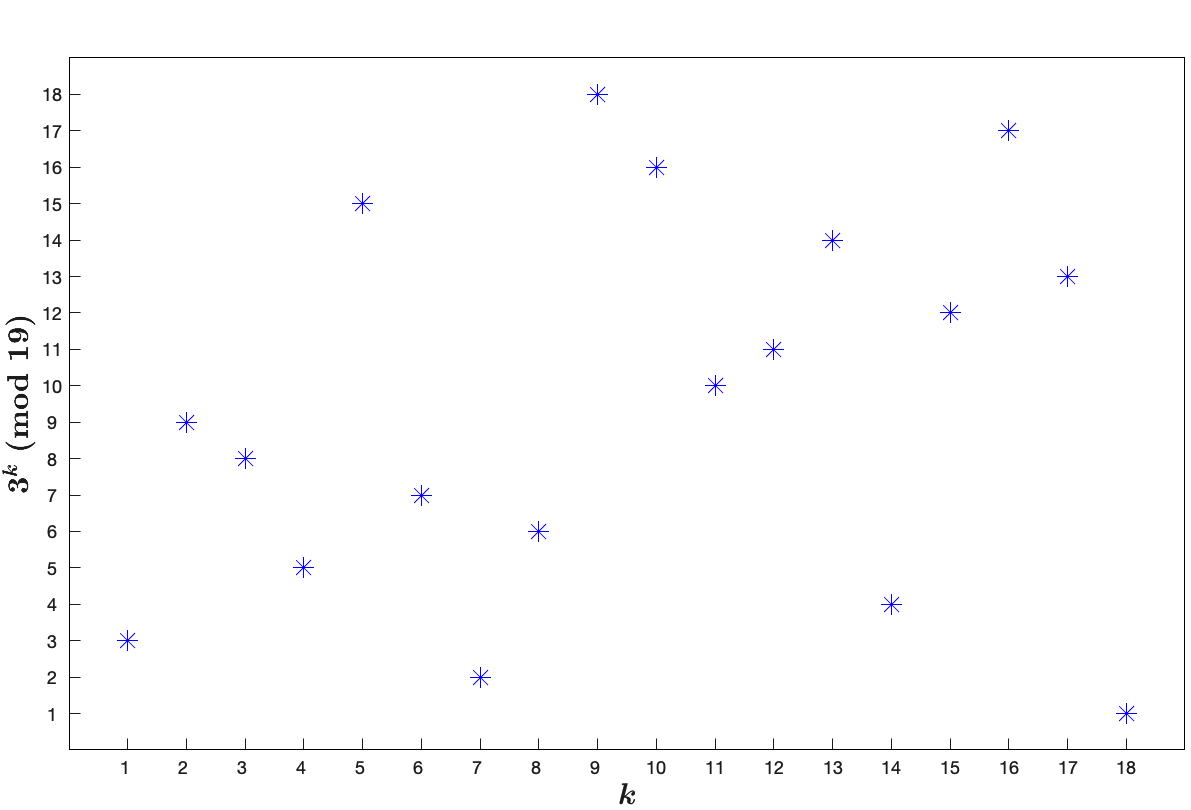
\includegraphics[width=1.25\textwidth]{graph3in19.png}
 	\caption[Example of the group structure of $GF(19)^\times$.]{Powers of the generator $g = 3$ in $GF(19)^\times$.}
 	\label{fig2}
 \end{figure}
\noindent Unfortunately, the function $g^k \text{ (mod 19)},\ k \in \mathbb{N},$ isn't monotonic. Therefore, we can't use the idea of trying a randomly selected $k_0$ and comparing $3^{k_0} \text{ (mod 19)}$ with $4$, but we can use the fact the group $G$ is finite and its order is $\#G = 18$. We can try all possible values of $k \in \{0, 1, \ldots, 17\}$ and find the solution. This method is called the \textbf{brute-force attack}. 
\begin{align*}
3^0 \equiv 1 \text{ (mod 19)} &\not\equiv 4 \text{ (mod 19)}, \\
3^1 \equiv 3 \text{ (mod 19)} &\not\equiv 4 \text{ (mod 19)}, \\
3^2 \equiv 9 \text{ (mod 19)} &\not\equiv 4 \text{ (mod 19)}, \\
3^3 \equiv 8 \text{ (mod 19)} &\not\equiv 4 \text{ (mod 19)}, \\
&\vdots \quad \vdots \\
3^{13} \equiv 14 \text{ (mod 19)} &\not\equiv 4 \text{ (mod 19)}, \\
3^{14} &\equiv 4 \text{ (mod 19)}.
\end{align*}
Therefore, the solution of this DLP is $k = 14$. We can see the brute-force approach is quite lengthy even for a DLP in a group of small order. The complexity of the brute-force attack in a group $G$ is $O(\#G)$ of group operations.
\begin{RM}
Standard properties of logarithms hold for discrete logarithms as well. Let $G$ be a finite Abelian group and let $g$ be a generator of $G$.
\begin{itemize}
\item $\forall p, q \in G: \log_g(pq) \equiv log_g(p) + log_g(q) \text{ (mod $\#G$)}$,
\item $\forall p, q \in G: \log_g(p(q)^{-1}) \equiv log_g(p) - log_g(q) \text{ (mod $\#G$)}$,
\item $\forall k \in \mathbb{Z},\ p \in G: \log_g(p^k) \equiv k \cdot log_g(p) \text{ (mod $\#G$)}$,
\item $h \in G,\ \langle h \rangle = G,\ \forall p \in G: log_g(p) \equiv log_h(p) \cdot log_g(h)  \text{ (mod $\#G$)}$.
\end{itemize}
Last property is the well-known change-of-base formula. That tells us that if we can solve the DLP with respect to some base effectively, we can use it to solve the DLP with respect to any other base effectively.
\end{RM}

\noindent The discrete logarithm problem can be stated in any group. The difficulty of solving it greatly depends on the group structure and the group operation. To solve the DLP, we can develop a generic algorithm that works in any group and doesn't explore the group structure. Alternatively, we can develop a specialised algorithm to tackle the DLP in a specific type of group. \\\\
\noindent For example, in an additive group $(\{0,1,\ldots, p-1\}, +_p)$, $p$ prime, we can solve the DLP in $O(\log^2(p))$ group operations using the EEA. In 1997, Victor Shoup proved that a generic algorithm to solve the DLP in a generic group of prime order $p$ has to do $O(\sqrt{p})$ group operations~\cite{shoup}. The best generic algorithm to match this lower bound is Pollard's $\rho$ (rho)-algorithm, described in subsection \ref{rhoText}. 
\\
\\
\noindent The main focus of this thesis is to solve the DLP stated on an elliptic curve using a specialised algorithm. 
\begin{DF}
Let $E$ be an elliptic curve over a prime field $GF(p)$, let $P$ be a generator of $E$ and let $Q$ be another point on $E$. \textbf{Elliptic curve discrete logarithm problem (ECDLP)} is to find an integer $k \in \{0,1,\ldots, \#E(p) - 1\}$, such that $Q = kP$.
\end{DF}
\section{Generic Algorithms for Solving ECDLP}
In this section, we present the three most known generic algorithms for solving the DLP, we use elliptic curves notation. The first algorithm is based on collision finding, the time complexity matches the Shoup's lower bound, but the memory requirements are immense. All three algorithms in this section are based on~\cite{mky}.
\subsection{Baby-step Giant-step Algorithm}
\begin{DF}
\textbf{(Baby-step Giant-step (BSGS))}: Let $E(p)$ be an elliptic curve group over $GF(p)$, equipped with the operation $\oplus$, $P \in E$ its generator and $kP = Q \in G,\ k \in \{0, 1, \ldots, \#E - 1\}$, we denote the order of $E(p)$ by $N = \#E(p)$. We know, based on Hasse's theorem (\ref{hase}), for large $p$, $N$ is approximately $p$. Following algorithm solves the ECDLP in $O(\sqrt{N}) \approx O(\sqrt{p})$ group operations $\oplus$.
\begin{itemize}
\item Let $n = \mathlarger{\mathlarger{\mathlarger{\lceil}}} \sqrt{N} \mathlarger{\mathlarger{\mathlarger{\rceil}}}$, we pre-compute a list of length $n$ of multiples of $P$.
\item $0P = \mathcal{O}, P, 2P, \ldots, (n-1)P.$ \hfill (baby-step phase) \\
Afterwards, we generate multiples of $Q$ until the first collision, with the list generated in the baby-step phase, occurs.
\item $Q \oplus (0\cdot n \ominus P) = Q,\ Q \oplus (1\cdot n \ominus P),\ \ldots\ 2,\ Q \oplus ((n-1)\cdot n \ominus P).$\\
This stage is called the giant-step phase.
\item When the collision occurs for some $i,j$, such that $iP$ and $Q \oplus (j\cdot n \ominus P)$ are equal. We can solve the ECDLP and find the solution $k$:
\begin{align*}
iP = Q \oplus (j\cdot n \ominus P) \implies i &\equiv k + (-jn) \text{ (mod $N$)}, \\
k &\equiv i + jn \text{ (mod $N$)}.
\end{align*}
\end{itemize}
\noindent The algorithm is deterministic and is guaranteed to find the solution as it goes over all the possible values of $k$. Every integer in $\{0, 1, \ldots, N - 1\}$ can be expressed as $i + jn,\ n = \mathlarger{\mathlarger{\mathlarger{\lceil}}} \sqrt{N} \mathlarger{\mathlarger{\mathlarger{\rceil}}},\ i,j \in \{0,1,\ldots, n-1\}.$ 
For the efficient implementation, it's crucial to be able to find a collision in the pre-computed list effectively. Therefore, it's advisable to use a hash table, to store the elements generated in the baby-step phase, in order to achieve the constant time lookup. If that is satisfied, the algorithm's complexity is $O(\sqrt{N})$ of group operations and the space complexity is also $O(\sqrt{N})$.
\end{DF}
\noindent For example, let $E = E_{1,1}(29)$ be an elliptic curve group over $GF(29)$ defined by the elliptic curve equation $y^2 = x^3 + x + 1$. Let $P = (24,25)$ be a generator of $E$, and let $Q \in E$ be some other point, we want to find an integer $k$, such that $Q = kP.$ Order of $E$ is 36, so we set $n = 6$. The list of points pre-calculated in the baby-step phase is shown in table \ref{baby}.
\begin{table}[h]
\centering
\begin{tabular}{ |c||c|c|c|c|c|c| }
\hline
$i$ & 0 & 1 & 2 & 3 & 4 & 5\\ \hline
 $iP$ & $\mathcal{O}$ & $(24,25)$ &  $(6,7)$ & $(0,28)$ & $(10,24)$ & $\textbf{(28,12)}$ \\ \hline
\end{tabular}
\caption[List of points pre-calculated in the baby-step phase]{List of points pre-calculated in the baby-step phase.}
\label{baby}
\end{table}
This step depends only on the elliptic curve group $E$ and its generator $P$. Therefore, we can pre-calculate it only once and reuse for calculation of discrete logarithms of different points with respect to the same base point $P$. Let's solve the ECDLP in this group for $Q = (18,15)$. We iterate over the multiples of $Q$ and look for a collision with the pre-calculated list shown in table \ref{baby}.
\begin{center}
\begin{tabular}{ |c||c|c|c|c|c|c| }
\hline
$j$ & 0 & 1 & 2 & 3 & 4 & 5\\ \hline
 $Q\oplus(6j\ominus P)$ & $(18,15)$ & $(11,3)$ &  $(12,1)$ & $(8,17)$ & $\mathbf{(28,12)}$ & $(24,4)$ \\ \hline
\end{tabular}
\end{center}
We have found a collision for $j=4$ and $i=5$, found collision is highlighted in bold in both tables. Therefore:
$$
5P = Q\oplus(24\ominus P) \implies 4 \equiv k -24 \text{ (mod 36)} \implies k \equiv 29  \text{ (mod 36)}.
$$
We can easily verify that $29P = (18,15) = Q.$
\subsection{Pollard's $\boldsymbol\rho$-Algorithm} \label{rhoText}
\noindent The main drawback of the BSGS algorithm is its space complexity, it needs to store $\sqrt{\#E}$ elliptic curve points. To remedy this problem, in 1978, John Pollard published a different algorithm, which is called after him, the Pollard's~$\rho$-algorithm. It has the same time complexity as BSGS, yet the memory requirements are minimal. We first describe Pollard's idea in general, then show how it can be applied to solve the ECDLP.
\begin{DF}
\label{pol}
 \textbf{(Pollard's $\boldsymbol\rho$-algorithm)}: Let $S$ be a finite set of $N$ elements, let $f: S \to S$ be a function. Choose $x_0 \in S$ a starting point of the sequence defined by: $x_i = (\underbrace{f\circ f \circ \cdots \circ f}_\text{$i$-times})(x_0)$, then there exists $L \in \mathbb{N}$ such that:
 $$
 x_{2i} = x_i, \quad 1\leq i < L.
 $$
Set $S$ is finite, therefore for some $k \in \mathbb{N}_{< N},$ the sequence $x_0, x_1, \ldots, x_k$ has to contain a point that repeats twice in this sequence. We denote the first such point by $x_T$. It's clear that after the point $x_T$, the sequence is in a cycle of length $M$, where $T+M$ is the index of the second occurrence of the point $x_T$ in the sequence. To prove the existence of an integer $i$, such that $x_{2i} = x_i$, we start with the fact that $\forall k \in \{0, 1, \ldots, M-1\}: x_{T+k} = x_{T+k+M},$ which implies:
$$
\exists i \in \mathbb{N},\ T \leq i < T + M: 2i \equiv i \text{ (mod $M$)} \implies i\ |\ M.
$$
The argument is simple, in every sequence of $M$ consecutive integers there has is exactly one integer divisible by $M$. Therefore, we can see that the $L$, from the definition \ref{pol}, is in fact $L= T + M \leq N$. On average (with different choices of $x_0$ and function $f$) it takes $O(\sqrt{N})$ steps to obtain a collision with a probability over 50\% (based on the birthday paradox), for a thorough analysis see~\cite{polProb}. \\ \\
\noindent For a graphical illustration see figure \ref{rho}, the first point in the sequence that repeats itself twice is $x_3$. Therefore, we set $T = 3$. The length of the cycle is $M = 6$, because $x_T = x_3 = x_{3+6}$. The only integer in the set $\{3,4,5,6,7,8\}$ that is divisible by $M = 6$ is $6$, therefore $i=6$ and we can easily verify that $x_6 = x_{2*6} = x_{12}$. Figure \ref{rho} has a strong resemblance to the Greek letter $\rho$, hence the name of the algorithm.
 \begin{figure}[h]
 \centering
 \hspace*{-1cm}
 	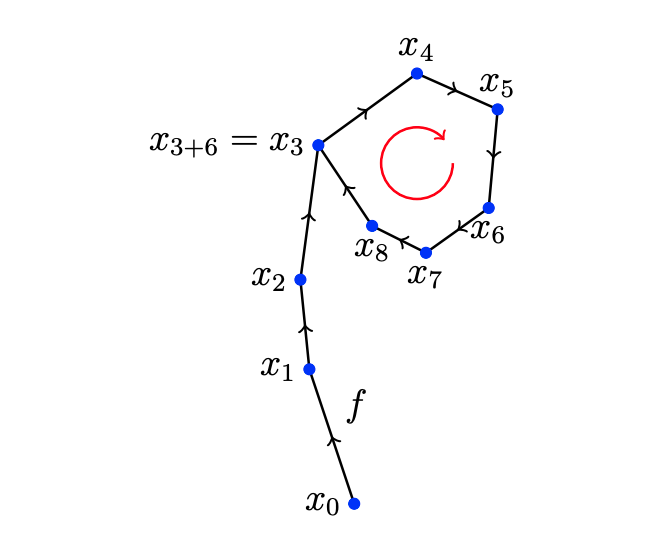
\includegraphics[width=1\textwidth]{rho.png}
 	\caption[Graphical illustration of the Pollard's $\rho$ collision idea]{Graphical illustration of the idea behind the Pollard's $\rho$-algorithm. $T = 3$, length of the cycle $M = 6$. Image source: (\cite{mky}, page $70$).}
 	\label{rho}
 \end{figure}
 \end{DF}
 \begin{DF}
 The Pollard's $\rho$-algorithm might be used to solve the ECDLP. Let $E(p)$ be an elliptic curve group over the finite field $\in GF(p)$. Let $P$ be a generator of $E(p)$, and let $Q \in E(p)$ be some other point. We want to find an integer $t=\log_P(Q)$. Let's denote the order of $E(p)$ by $N = \#E$. We divide $E$ into three disjunctive sets $S_1, S_2, S_3$ of approximately the same size. Additionally, we require that $\mathcal{O} \not\in S_2$. For $i \in \mathbb{Z}_{\geq 0}$ we define a function $f: E \to E$ as follows:
 $$
 T_{i+1} = f(T_i) := \begin{cases} P \oplus T_i,\quad T_i \in S_1, \\
 2T_i, \quad T_i \in S_2, \\
 Q \oplus T_i, \quad T_i \in S_3.
 \end{cases}
 $$
 We can start with any point in $E(p)$ as long as we know how to express it as a linear combination of points $P,Q$. The usual choice is $T_0 = \mathcal{O} = 0P + 0Q$. After $k$ steps we get:
 $$
 T_k = (\underbrace{f\circ f \circ \cdots \circ f}_\text{$k$-times}(\mathcal{O}) = \alpha_k P \oplus \beta_k Q.
 $$
 We need to keep track of $\alpha_k,\ \beta_k$. We start with integers $\alpha_0, \beta_0$, such that $\alpha_0P + \beta_0Q = T_0,$ and define the update process recursively.
\begin{align*}
 \forall k \in \mathbb{Z}_{\geq 0}:  \alpha_{k+1} := \begin{cases} \alpha_k + 1\text{ (mod $N$)},\quad &T_k \in S_1, \\
 2\alpha_k\text{ (mod $N$)}, \quad &T_k \in S_2, \\
 \alpha_k, \quad &T_k \in S_3.
 \end{cases} \\
   \forall k \in \mathbb{Z}_{\geq 0}: \beta_{k+1} := \begin{cases} \beta_k,\quad &T_k \in S_1, \\
 2\beta_k\text{ (mod $N$)}, \quad &T_k \in S_2, \\
 \beta_k + 1\text{ (mod $N$)}, \quad &T_k \in S_3.
 \end{cases}
 \end{align*}
We also create a second sequence of points on the elliptic curve $E$: 
$$\forall k \in \mathbb{Z}_{\geq 0}: R_k := T_{2k} = \gamma_kP \oplus \delta_kQ.$$
After some number of steps, let's denote it by $i$, we encounter a collision: $R_i = T_i$. Then we have a relation: 
$$
\gamma_iP \oplus \delta_iQ = \alpha_iP \oplus \beta_iQ.
$$
Let $d = \text{gcd}(\beta_i - \delta_i, N)$, if $d=1$ we can easily find the solution $t$ to the ECDLP:
$$
t \equiv (\gamma_i - \alpha_i)\cdot(\beta_i - \delta_i)^{-1} \text{ (mod $N$)}.
$$
If $d \neq 1$, but is small, it might be favourable to find a particular solution $y$ mod($N/d$) in the same fashion:
$$
y \equiv (\gamma_i - \alpha_i)\cdot(\beta_i - \delta_i)^{-1} \text{ $\bigg($mod $\frac{N}{d}\bigg)$}.
$$
Afterwards, we can recover the complete solution $t$ from the set:
$$
\bigg\{y + k\cdot\frac{N}{d}\ \bigg| \ k \in \{0, 1, \ldots, d -1\}\bigg\}.
$$
For $N$ prime $d$ will be small, if $d$ is not small, we can restart the algorithm with a different partitioning $S_1,S_2,S_3$ or a different starting point $T_0$. Another option is to use the Pohlig-Hellman algorithm and solve multiple ECDLPs in prime subgroups. Then find the complete solution $t$ using the Chinese remainder theorem (CRT).
\end{DF}
\noindent For example, let $E = E_{11,18}(29)$ be an elliptic curve group over $GF(29)$, defined by the elliptic curve equation is $y^2 = x^3 + 11x + 18$. Let $P = (1,1)$ be a generator of $E$, and let $Q \in E$ be a second point, we want to find an integer $t$ such that: $Q = tP.$
Order of $E$ is 29 (prime). We divide points in $E$ into sets $S_1,S_2,S_3$ based on their $x$-coordinates (assume $x$-coordinate of $\mathcal{O}$ is $0$):
\begin{align*}
\forall R = (R_x, R_y) \in E: \begin{cases} R \in S_1, \quad \text{ if } 0 &\leq R_x < \big\lfloor\frac{p}{3}\big\rfloor, \\ 
R \in S_2, \quad \text{ if } \big\lfloor\frac{p}{3}\big\rfloor &\leq R_x < 2\big\lfloor\frac{p}{3}\big\rfloor, \\
R \in S_3, \quad \text{ if } 2\big\lfloor\frac{p}{3}\big\rfloor &\leq R_x, 
\end{cases}
\end{align*}
where $p = 29.$ 
Set $S_1$ contains the identity element $\mathcal{O}$. Cardinalities of the sets are $|S_1| = 9,\ |S_2| = 12, \ |S_3| = 8.$ There are many different ways how to divide the points in $E$ into sets $S_1,S_2,S_3$. The important thing here is, the three sets are approximately of the same size. Also, for every point $R \in E$ we can efficiently decide to which of the three sets it belongs. \\ \\
\noindent Let's solve the ECDLP with $Q=(13,26)$. In the table \ref{tblRho} are shown the intermediate results of the Pollard's $\rho$-2algorithm.
\begin{table}[!h]
\centering
\begin{tabular}{ |c||c|c|c|c|c|c| } 
\hline
$i$ & $\alpha_i$ & $\beta_i$ & $T_i$ & $\gamma_i$ & $\delta_i$ & $R_i$ \\ 
\hline
\hline
0 & 0 & 0 & $\mathcal{O}$ &  0 & 0 & $\mathcal{O}$ \\ \hline
1 & 1 & 0 & $(1,1)$ &  2 & 0 & $(18,25)$ \\ \hline
2 & 2 & 0 & $(18,25)$ &  3 & 1 & $(3,22$ \\ \hline
3 & 2 & 1 & $(5,13)$ &  8 & 2 & $(11,7)$ \\ \hline
4 & 3 & 1 & $(3,22)$ &  3 & 8 & $(8,3)$ \\ \hline
5 & 4 & 1 & $(12,14)$ &  4 & 9 & $(13,3)$ \\ \hline
6 & 8 & 2 & $(11,7)$ &  8 & 19 & $(13,3)$ \\ \hline
7 & 16 & 4 & $(14,4)$ &  16 & 10 & $(13,3)$ \\ \hline
8 & 3 & 8 & $(8,3)$ &  3 & 21 & $(13,3)$ \\ \hline
9 & 4 & 8 & $(26,25)$ &  6 & 14 & $(13,3)$ \\ \hline
10 & 4 & 9 & $\mathbf{(13,3)}$ &  12 & 0 & $\mathbf{(13,3)}$ \\ \hline
\end{tabular}
\caption[Intermediate values of the Pollard's $\rho$-algorithm]{Intermediate values of the Pollard's $\rho$-algorithm.}
\label{tblRho}
\end{table}
\\
\noindent A collision was found after 10 iterations: 
$$
4P + 9Q = 12P \implies t \equiv 8\cdot9^{-1} \text{ (mod $29$)} \equiv 17 \text{ (mod $29$)}. 
$$
We can easily verify that $17P = (13,26) = Q.$
\subsection{Pohlig-Hellman Algorithm}
As we have mentioned in the previous subsection, Pollard's $\rho$-algorithm works best in a prime order group. In a case, when the order of a group $G$ is a composite number $N$ with small factors, we can solve multiple ECDLPs in subgroups of prime order. Then, we can use the CRT to find the complete solution. In 1978, Stephen Pohlig and Martin Hellman presented this algorithm in their article~\cite{PH}. 
\begin{DF} (\textbf{Chinese Remainder Theorem (CRT))}: Let $m_i \in \mathbb{N},\ i \in \{1,\ldots, k\},$ be mutually prime integers, and $N=\prod_{i=1}^k m_i,\ x_i \in \mathbb{Z},\ i \in \{1,\ldots, k\}.$ 
The following system of linear congruences:
\begin{align*}
x &\equiv x_1 \text{ (mod $m_1$)}, \\
x &\equiv x_2 \text{ (mod $m_2$)}, \\
&\vdots \quad \vdots \\
x &\equiv x_k \text{ (mod $m_k$)},
\end{align*}
has a solution $c$:
$$
c = \sum_{i=1}^k x_iN_iM_i \text{ (mod $N$)},
$$ where $N_i=N/m_i$ and $M_i\equiv(N_i)^{-1} \text{ (mod $m_i$)}$. Moreover, any other solution $c'$ is congruent to $c$ modulo $N$.
\end{DF}
\begin{DF}(\textbf{Pohlig-Hellman algorithm}): Let $E(p)$ be an elliptic curve group of composite order $N$ and let the factorisation of $N$ be:
$$
N = \prod_{i=1}^kp_i^{e_i},\ \forall i,j \in \{1, 2, \ldots, k\}: e_i \in \mathbb{Z}_{\geq 0},
$$ where $p_i$ are distinct primes. Let $P$ be a generator of $E(p)$ and let $Q \in E(p)$. We want to find an integer $x$, such that $xP = Q$. We can split this ECDLP into multiple ECDLPs in a prime power subgroups as follows:
 \begin{itemize}
 \item For each $i \in \{1, 2, \ldots, k\}$ let:
 $$
 P_i := \frac{N}{p_i^{e_i}}P, \quad Q_i := \frac{N}{p_i^{e_i}}Q.
 $$ Each $P_i$ is a generator of a prime power subgroup of $E(p)$. Order of $P_i$ is $\#P_i = p_i^{e_i}.$ We solve an ECDLP in every subgroup $\langle P_i \rangle$, i.e. find an integer $x_i$  such that: $x_iP_i = Q_i.$
 \item  In every prime power subgroup $\langle P_i \rangle$, we may split the ECDLP to $e_i$ ECDLPs in prime subgroups of order $p_i$.  We may rewrite the unknown integer $x_i := y_{i,0} + y_{i,1}p_i + y_{i,2}p_i^2+ \cdots + y_{i,e-1}p_i^{e_i-1}.$ We can now repeatedly solve an ECDLP in a prime subgroup to obtain one unknown digit of $x_i$ at a time, by shifting the rest of them out. To find the first digit $y_{i,0}$ multiply both sides of the equation by $p_i^{e_i-1}$:
\begin{align*}
p_i^{e_i-1} Q_i &= p_i^{e_i-1}\cdot x_i  P_i\\ 
&= p_i^{e_i-1}\cdot (y_{i,0} + y_{i,1}p_i + y_{i,2}p_i^2+ \cdots + y_{i,e-1}p_i^{e_i-1})P_i \\
&= p_i^{e_i-1}y_{i,0}P_i \oplus p_i^{e_i}\cdot\underbrace{(y_{i,1} + y_{i,2}p_i+ \cdots + y_{i,e-1}p_i^{e_i-2})P_i}_{\in \langle P_i \rangle} \\
&= y_{i,0}p_i^{e_i-1}P_i, \quad \text{(because }\forall T \in \langle P_i \rangle : p_i^{e_i}T = \mathcal{O})
\end{align*}
We may now solve the ECDLP in a prime subgroup of order $p_i$ generated by $p_i^{e_i-1}P_i$, and obtain the first digit $y_{i,0}.$ Afterwards, we move to the next digit $y_{i,1}$ and find it in a similar fashion.
\begin{align*}
p_i^{e_i-2} Q_i &= p_i^{e_i-2}\cdot x_i  P_i\\ 
&= p_i^{e_i-2}\cdot (y_{i,0} + y_{i,1}p_i + y_{i,2}p_i^2+ \cdots + y_{i,e-1}p_i^{e_i-1})P_i \\
&= (p_i^{e_i-2}y_{i,0} + p_i^{e_i-1}y_{i,1})P_i \oplus p_i^{e_i}\cdot\underbrace{y_{i,2}+ \cdots + y_{i,e-1}p_i^{e_i-3})P_i}_{\in \langle P_i \rangle} \\
&= y_{i,0}p_i^{e_i-2}P_i \oplus y_{i,1}p_i^{e_i-1}P_i \implies \\
p_i^{e_i-2}(Q_i \ominus y_{i,0}P_i) &= y_{i,1}p_i^{e_i-1}P_i.
\end{align*}
To the digit $y_{i,1}$, we need to solve the ECDLP in a prime subgroup of order $p_i$. We continue in the same fashion until all digits of $x_i$ are recovered.
\item Finally we solve the following system of linear congruences.
\begin{align*}
x &\equiv x_1 \text{ (mod $p_1^{e_1}$)}, \\
x &\equiv x_2 \text{ (mod $p_2^{e_2}$)}, \\
&\vdots \quad \vdots \\
x &\equiv x_k \text{ (mod $p_k^{e_k}$)},
\end{align*}
using the CRT to obtain the complete solution $x$.
\end{itemize}
\end{DF}
\noindent In the individual phase, when we are solving the ECDLP in a prime order subgroup we can use any algorithm. Usually, the BSGS or Pollard's $\rho$-algorithm is used. The time complexity of Pohlig-Hellman algorithm is therefore (for more information see~\cite{mky}):
$$
O\bigg(\sum_{i=1}^k\bigg[e_i\big(S(p_i) + \log(p_i)\big)\bigg]\bigg),
$$ where $S(p_i)$ is the time complexity of the algorithm used to solve the ECDLP in the prime subgroup of order $p_i$. For elliptic curve groups of composite order with small factors is Pohlig-Hellman significantly faster than the BSGS or Pollard's $\rho$-algorithm (we often need to run it more than once with different starting points if the group order is a composite number). \\\\
\noindent For example, let $E = E_{1,2}(75941)$ be an elliptic curve over the finite field $GF(75941)$, defined by the elliptic curve equation $y^2 = x^3 + x + 2$. Let $P = (64579,62139)$ be a generator of $E$, let $Q \in E$ be a point on the elliptic curve $E$, we want to find an integer $x$, such that $Q = xP.$ Order of $E$ is $76428 = 2^2\cdot 3^2\cdot 11 \cdot 193$. Let's solve the ECDLP for $Q = (1447, 50835)$. \\ \\
\noindent We show how can the Pohlig-Hellman algorithm solve this ECDLP. 
\begin{table}[H]
\centering
\begin{tabular}{ |c||c|c|c|c|c| } 
\hline
 $i$ & $p_i$ & $e_i$ & $P_i$ & $Q_i$ & $x_i$  \\
\hline
\hline
1 & 2 & 2 & $19107P = (1, 75939)$ &  $19107Q = (1,2)$ & 3  \\ \hline
2 & 3 & 2 & $8492P = (55693, 45178)$ &  $8492Q = (17273,40444)$ & 2 \\ \hline
3 & 11 & 1 & $6948P = (39499, 25804)$ &  $6948Q = (29264,5197)$ & 9 \\  \hline
4 & 193 & 1 & $396P = (58124, 73147)$ &  $396Q = (34502,8697)$ & 189 \\ \hline
\end{tabular}
\caption[Intermediate values of the Pohlig-Hellman algorithm]{Intermediate values of the Pohlig-Hellman algorithm.}
\label{tblPH}
\end{table}
\noindent For $i=1,2$ we need to solve an ECDLP in a subgroup of prime power order. In the subgroup of order $2^2$, generated by $P_1 = (1, 75939)$. We rewrite the unknown partial solution $x_1$ as $x_1 = y_{1,0} + 2y_{1,1}$. We use the following equation to find the first digit $y_{1,0}$.
\begin{align*}
2Q_1 &= y_{1,0}\cdot2P_1 \\
(75940, 0) &= y_{1,0}(75940, 0) \implies y_{1,0} = 1.
\end{align*}
To recover the second digit $y_{1,1}$, we proceed in the similar fashion.
\begin{align*}
Q_1 \ominus y_{1,0}\cdot P_1 &= y_{1,1}\cdot 2P_1 \\
(1,2) \oplus (1,2) & = y_{1,1}(75940, 0) \\
(75940, 0) &= y_{1,1}(75940, 0) \implies y_{1,1} = 1.
\end{align*}
Therefore, $x_1 = y_{1,0} + y_{1,0}\cdot 2 = 1 + 2 = 3.$ In reality, we could have just tried all four possible values for $x_1$. \\ \\
\noindent We repeat the whole process in the subgroup of order $3^2$ generated by $P_2 = (55693, 45178)$. We rewrite the unknown partial solution $x_2$ as $x_2 = y_{2,0} + 3y_{2,1}$, and use the following equation to find the first digit $y_{2,0}$.
\begin{align*}
3Q_2 &= y_{2,0}\cdot 3P_2 \\
(35655, 11621) &= y_{2,0}(35655, 64320) \implies y_{2,0} = 2.
\end{align*}
To find the second digit $y_{2,1}$, we proceed in the similar fashion.
\begin{align*}
Q_2 \ominus y_{2,0}\cdot P_2 &= y_{2,1}\cdot 3P_2 \\
Q_2 \ominus 2P_2 &= y_{2,1}\cdot (35655, 64320) \\
\mathcal{O} &= y_{2,1}\cdot (35655, 64320) \implies y_{2,1} = 0.
\end{align*}
Therefore, $x_2 = 2 + 0\cdot 3 = 2$. In this case, there are nine possible values for $x_2$, which could all have been tried out in the blink of an eye. \\\\
\noindent Now we assemble the system of linear congruences and solve it to find the complete solution $x$.
\begin{align*}
x &\equiv 3 \text{ (mod $4$)}, \\
x &\equiv 2 \text{ (mod $9$)}, \\
x &\equiv 9 \text{ (mod $11$)}, \\
x &\equiv 189 \text{ (mod $193$)}, \\
\end{align*}
\begin{table}[!h]
\centering
\begin{tabular}{ |c||c|c|c|c| } 
\hline
 $i$ & $x_i$ & $m_i$ & $N_i$ & $M_i$ \\
\hline
\hline
1 & 3 & 4 & 19107 &  3 \\ \hline
2 & 2 & 9 & 8492 & 2\\ \hline \hline
3 & 9 & 11 & 6948 & 8 \\ \hline
4 & 189 &193 & 396 & 58 \\ \hline
\end{tabular}
\caption[CRT phase of Pohlig-Hellman algorithm]{Intermediate values of the CRT phase of the Pohlig-Hellman algorithm.}
\label{tblPH3}
\end{table}
\noindent Using the CRT, we compute $x$ (the intermediate values are in table \ref{tblPH3}).
\begin{align*}
x &\equiv 3\cdot 19107 \cdot 3 + 2\cdot 8492 \cdot 2 +  9\cdot 6948 \cdot 8 +  189\cdot 396 \cdot 58 \text{ (mod  76428)}\\
 &\equiv 2891\text{ (mod  76428)}.
\end{align*}
We can easily verify that $2891P = (1447, 50835) = Q.$
\section{Index Calculus for ECDLP}
The Index Calculus is originally a \textbf{subexponential} algorithm for solving the DLP in a multiplicative group of a finite field. 
\begin{DF}
Let $0\leq a \leq 1,\ a \in \mathbb{R}$ and $c \in \mathbb{R}_{>0}$. The \textbf{subexponential function} for the parameters $a$ and $c$ is:
$$
L_N(a,c) := \exp(c\log(N)^a \log(\log(N))^{1-a}).
$$
Let $N$ be a $k$-bit integer, note that taking $a=0$ gives $L_N(0,c) = \log(N)^c = k^c$ (polynomial), while taking $a=1$ gives $L_N(1,c) = N^c = \exp(ck)$ (exponential). Thus, $L_N(a,c)$ interpolates exponential and polynomial growth. An algorithm is called \textbf{subexponential} when it's complexity is $O(L_N(a,c))$ for some $a$, $0 < a < 1$. For more information see chapter 15 in~\cite{subExp}.
\end{DF} 
\noindent However, it's common to use the name index calculus algorithm to refer to any algorithm, that operates in the same fashion as the original Index Calculus algorithm. In other words, that solves the DLP by first collecting relations between the group elements, and then using linear algebra~\cite{amadori17}.
\begin{DF}
\textbf{Index Calculus for ECDLP}: Let $E(p)$ be an elliptic curve over a prime order field $GF(p)$, let $P$ be a generator of $E(p)$. For simplicity, we assume $\#P$ is prime, if that's not the case, we can use the Pohlig-Hellman idea to split the ECDLP into multiple ECDLPs in prime order subgroups. Let $Q \in E$ be another point, we want to find an integer $x$, such that $xP = Q$. The simplest version of the index calculus algorithm consists of two main stages, the relation collection step and the linear algebra step. First, we need to collect relations.
\begin{enumerate}
\item Specify a factor base $\mathcal{F} \subset E$, such that we can effortlessly test the membership of an element to this factor base. 
\item Generate a random linear combination $R$ of points $P,Q$.
$$
R := uP + vQ,\quad \text{$u,v$ are random integers in $GF(\#P)$}.
$$
\item If possible, express $R$ as a linear combination of the elements of the factor base $\mathcal{F}$:
\begin{align*}
&\forall k \in \{1,2,\ldots,|\mathcal{F}|\}: P_k \in \mathcal{F},\ a_k \in GF(\#P): \\
&R = uP + vQ = \sum_{k=1}^{|\mathcal{F}|}a_k P_k, \\
&\mathcal{O} = -uP - vQ + \sum_{k=1}^{|\mathcal{F}|}a_k P_k.
\end{align*}
\item If $R$ cannot be expressed in terms of the factor base $\mathcal{F}$, continue with step 2. Otherwise, store the coordinates of $R$ with respect to $\mathcal{F}$ and integers $u,v$ as a row in the relation matrix $M$. The row is stored in this form:
$$
(a_1, a_2, \ldots, a_{|\mathcal{F}|}, -u, -v).
$$
\item We repeat this procedure (steps 2 to 4) until the end condition is met.
\noindent Some authors (see~\cite{amadori17} page 2) suggest, to set the end condition to the number of decomposed points $R$ to be at least $|\mathcal{F}|$. However, we need to state this condition doesn't guarantee the obtained relations are enough to solve the ECDLP. Another option, which guarantees we can solve the ECDLP in the next step, is to collect relations until the rank of the matrix $M$ is $|\mathcal{F}| + 1$. Which is also the maximum rank, matrix $M$ can have (assuming $Q \neq \mathcal{O}$). We will state a weaker, that usually requires fewer relations to be found, end condition in section \ref{alg1}. 
\\ \\
\noindent After collecting enough relations, the linear algebra step solves the ECDLP.
\item We reduce matrix $M$ to a row echelon form (definition \ref{rowEch}). Then, the last non-zero row of the reduced matrix looks like $(0,0,\ldots, 0, 1, -v')$, which transforms into the following relation.
\begin{align*}
\mathcal{O}  &= 1P \oplus (-v'Q) \\
P &= v'Q \implies x \equiv (v')^{-1} \text{ (mod $\#P$)}.
\end{align*}
We can always recover the solution $x$ because the order of $\#P$ is prime and $P \neq \mathcal{O} \implies v' \not\equiv 0 \text{ (mod $\#P$)}$.
\end{enumerate}
\end{DF}
\noindent The main bottleneck of this algorithm lies in the decomposition of a point $R$ into the factor basis $\mathcal{F}$, called the \textbf{point decomposition problem (PDP)}. Therefore, in order for this algorithm to be efficient, we need to be able to efficiently solve the PDP (including the case when $R$ can't be decomposed into the elements of $\mathcal{F}$). Additionally, we require a high success rate of the decomposition of $R$ into the factor base $\mathcal{F}$. Both these requirements are deeply affected by choice of the factor base $\mathcal{F}$ and its size~\cite{amadori17}. \\ 

\subsection{Summation Polynomials}
\noindent In 2004, Igor Semaev published an article introducing summation polynomials in order to transform the PDP to a problem of finding a solution of a multivariate polynomial equation based on the group law of a specific elliptic curve. This section is based on the original article by Semaev~\cite{semaev04}.
\begin{DF}
Let $E_{A,B}(p)$ be an elliptic curve given by the short Weierstrass equation over a prime field $\mathbb{F} = GF(p),\ p > 3$. For any natural number $n \geq 2$, let $S_n = S_n(X_1, X_2, \ldots, X_n)$ be a polynomial in $n$ variables, which is related to the group operation on $E_{A,B}(p)$. We call this polynomial the $n$-th \textbf{summation polynomial} and define it by the following property. Let $x_1,x_2,\ldots,x_n$ be any elements in $\overline{\mathbb{F}}$, the algebraic closure of the field $\mathbb{F}$, then $S_n(x_1,x_2,\ldots,x_n)=0$ if and only if there exist $y_1,y_2,\ldots,y_n \in \overline{\mathbb{F}}$, such that the points $(x_i,y_i), \forall i \in \{1,2,\ldots,n\}$, are in $E(\overline{\mathbb{F}})$, and sum to the identity element of $E_{A,B}(\overline{\mathbb{F}})$.
$$
\sum_{i=1}^n (x_i,y_i) = \mathcal{O}, \quad  \mathcal{O} \in E_{A,B}(\overline{\mathbb{F}}).
$$
For $n=2$, the summation polynomial is defined as follows. 
$$
S_2(X_1, X_2) := X_1 - X_2,
$$ it comes from the fact that 
$$
\forall P, Q \in E_{A,B}(\overline{\mathbb{F}}): P \oplus Q = \mathcal{O} \implies  Q = \ominus P.
$$
Based on the definition of the additive inverse in $E_{A,B}(\overline{\mathbb{F}})$, we know, the points $P = (x_1,y_1)$ and $\ominus P = (x_1, -y_1)$ have the same $x$-coordinate. Which is equivalent to $S_2(x_1, x_2) = 0 \implies x_1 = x_2.$ 
\\\\
\noindent To determine $S_3(X_1,X_2,X_3),$ let $(x_1,y_1)$ and $(x_2, y_2)$ be two affine ($\neq  \mathcal{O}$) points on $E_{A,B}(\overline{\mathbb{F}})$, such that $x_1 \neq x_2.$ We denote their sum and difference by:
\begin{align*}
(x_3,y_3) &:= (x_1,y_1) \oplus (x_2,y_2),\\
(x_4,y_4) &:= (x_1,y_1) \ominus (x_2,y_2).\\
\end{align*}
We use the group law $\oplus$ to express $x_3$ and $x_4$ in terms of $x_1,x_2, y_1, y_2$.
\begin{align*}
x_3 &= \lambda_3^2 - (x_1 + x_2), \text{ where } \lambda_3 = \frac{y_2 - y_1}{x_2 - x_1},\\ 
x_4 &= \lambda_4^2 - (x_1 + x_2), \text{ where } \lambda_4 = \frac{y_2 + y_1}{x_2 - x_1}, \text{ since } \ominus (x_2,y_2) = (x_2, -y_2),\\ 
\end{align*}
To find a polynomial, such that $x_3$ and $x_4$ are its roots, recall \textbf{Vieta's formulas}, let $z_1, z_2$ be two roots of a polynomial $p(z) = az^2 + bz + c$. Then the following formulas must be satisfied:
$$
z_1 + z_2 = -\frac{b}{a},\quad z_1z_2 = \frac{c}{a}.
$$
Therefore, we want to express $x_3 + x_4$ and $x_3 x_4$ in terms of $x_1,x_2,A,B$.
\begin{align*}
x_3 + x_4 &= \lambda_3^2 + \lambda_4^2 - 2(x_1+x_2) \\
&= \frac{(y_2-y_1)^2 + (y_2+y_1)^2 -2(x_1+x_2)(x_2-x_1)^2}{(x_2-x_1)^2} \\
&= \frac{2y_2^2+2y_1^2 -2(x_1+x_2)(x_2-x_1)^2}{(x_2-x_1)^2}.
\end{align*}
Substitute for $y_1^2,y_2^2$ using the elliptic curve equation $Y^2 = X^3 + AX + B.$
 \begin{align*}
x_3 + x_4 &= \frac{2(x_1^3+Ax_1+B+x_2^3+Ax_2+B) -2(x_1^3+x_2^3-x_1^2x_2-x_1x_2^2)}{(x_2-x_1)^2},\\
&= 2\frac{(Ax_1+Ax_2+2B) +x_1^2x_2+x_1x_2^2}{(x_2-x_1)^2}, \\
&= 2\frac{x_1(x_1x_2 + A) + x_2(x_1x_2 + A)+2B}{(x_2-x_1)^2},\\ 
&= 2\frac{(x_1 + x_2)(x_1x_2 + A)+2B}{(x_2-x_1)^2}.
\end{align*}
\vphantom{.}
\begin{align*}
\mathsmaller{x_3x_4} &= \mathsmaller{\frac{\big((y_2-y_1)^2 -(x_1^3+x_2^3-x_1^2x_2-x_1x_2^2)\big)\big((y_2+y_1)^2-(x_1^3+x_2^3-x_1^2x_2-x_1x_2^2)\big)}{(x_2-x_1)^4}}, \\
&= \mathsmaller{\frac{\big(y_1^2 + y_2^2 -2y_1y_2 -x_1^3-x_2^3+x_1^2x_2+x_1x_2^2\big)\big(y_1^2 + y_2^2 +2y_1y_2 -x_1^3-x_2^3+x_1^2x_2+x_1x_2^2\big)}{(x_2-x_1)^4}},\\
&= \mathsmaller{\frac{\big(x_1^2x_2 + x_1x_2^2 + Ax_1 + Ax_2 - 2y_1y_2 + 2B\big)\big(x_1^2x_2 + x_1x_2^2 + Ax_1 + Ax_2 + 2y_1y_2 + 2B\big)}{(x_2-x_1)^4}},\\
&= \mathsmaller{\frac{- 4 y_{1}^{2} y_{2}^{2} + x_{1}^{2} x_{2}^{4} + 2 x_{1}^{3} x_{2} A + 4 x_{1}^{2} x_{2}^{2} A + 2 x_{1} x_{2}^{3} A + x_{1}^{2} A^{2} + 2 x_{1} x_{2} A^{2} + x_{2}^{2} A^{2}}{(x_2-x_1)^4}} \\
&+\mathsmaller{ \frac{4 x_{1}^{2} x_{2} B + 4 x_{1} x_{2}^{2} B + 4 x_{1} A B + 4 x_{2} A B + 4 B^{2} + x_{1}^{4} x_{2}^{2} + 2 x_{1}^{3} x_{2}^{3}}{(x_2-x_1)^4}}.
\end{align*}
\vphantom{.}
Substitute for $y_1^2,y_2^2$ using the elliptic curve equation $Y^2 = X^3 + AX + B.$\\
\vphantom{.}
\begin{align*}
x_3x_4 &= \frac{\bigg((x_1-x_2)^2\bigg)\bigg(x_{1}^{2} x_{2}^{2} - 2 x_{1} x_{2} A + A^{2} - 4 x_{1} B - 4 x_{2} B\bigg)}{(x_2-x_1)^4},\\
&= \frac{(x_1x_2-A)^2 - 4B(x_1+x_2)}{(x_2-x_1)^2}.
\end{align*}
Therefore, the $x_3$ and $x_4$ are roots of the polynomial $f(X)$.
\begin{align*}
f(X) :=& (x_2-x_1)^2X^2-2\bigg((x_1+x_2)(x_1x_2 + A) + 2B\bigg)X \\
+& \bigg((x_1x_2-A)^2 - 4B(x_1+x_2)\bigg).
\end{align*}
In the case $x_1=x_2$, one of the points $(x_3,y_3),\ (x_4,y_4)$ is $2(x_1,y_1)$ and the other one has to be $\mathcal{O}$. Without loss of generality, let's consider $(x_3,y_3) = 2(x_1,y_1)$, we show that $x_3$ is the root of the polynomial $f(X)$.
\begin{align*}
x_1 = x_2:\ f(X) &= -2\bigg(2x_1(x_1^2+A)+2B\bigg)X +\bigg((x_1^2-A)^2-8Bx_1\bigg),
\\ X &= \frac{(x_1^2-A)^2-8Bx_1}{4(x_1^3+Ax_1+B)}, \\ 
	X &= \frac{x_1^4-2Ax_1^2-8Bx_1+A^2}{4(x_1^3+Ax_1+B)}.
\end{align*}
Let's express $x_3$ in terms of $x_1,x_2,A,B$.
\begin{align*}
\lambda &= \frac{3x_1^2+A}{2y_1}, \\
	x_3 &= \lambda^2 -2x_1, \\
	x_3 &= \frac{9 x_{1}^{4} + 6 Ax_{1}^{2} + A^{2} -8x_1y_1^2}{4y_1^2}.
\end{align*}
Substitute for $y_1^2$ using the elliptic curve equation $Y^2 = X^3 + AX + B.$
\begin{align*}
x_3 &= \frac{9 x_{1}^{4} + 6A x_{1}^{2} + A^{2}-8 x_{1}^{4} - 8 x_{1}^{2} A - 8B x_{1}}{4(x_1^3+Ax_1+B)} \\
x_3 &= \frac{x_1^4-2Ax_1^2 - 8Bx_1+ A^2}{4(x_1^3+Ax_1+B)}.\\
\end{align*}
The root of $f(X)$ is indeed $x_3$.
Therefore, we define the third summation polynomial as follows:
\begin{align*}
S_3(X_1,X_2,X_3) &:= (X_2-X_1)^2X_3^2-2\bigg((X_1+X_2)(X_1X_2 + A) + 2B\bigg)X_3\\
&+ (X_1X_2-A)^2 - 4B(X_1+X_2).
\end{align*}
$S_3$ is a symmetric polynomial of degree $2$ in each variable $X_1,X_2,X_3$. For more information about summation polynomials see~\cite{semaev04}. In the same article, Semaev also defined a general $n$-th summation polynomial as follows:
\begin{align*}
&\forall k,n \in \mathbb{N},\ n \geq 4,\ n-3\geq k \geq 1:\\
&S_n(X_1,X_2,\ldots, X_n) := \text{Res}_y\bigg(S_{n-k}(X_1,\ldots,X_{n-k-1},y),\ S_{k+2}(X_{n-k},\ldots,X_n,y)\bigg).
\end{align*}
For example, 
\begin{align*}
S_4(X_1,X_2,X_3,X_4) &= \text{Res}_y\bigg(S_3(X_1,X_2,y),\ S_3(X_3,X_4,y)\bigg), \\
S_3(X_1,X_2,y) &= c_0y^2 + c_1y + c_2, \text{ where } \\
c_0 &= (X_2-X_1)^2,\\ 
c_1 &= -2\bigg((X_1+X_2)(X_1X_2 + A) + 2B\bigg),\\
c_2 &=  (X_1X_2-A)^2 - 4B(X_1+X_2),  \\
S_3(X_3,X_4,y) &= d_0y^2 + d_1y + d_2, \text{ where } \\
d_0 &= (X_4-X_3)^2,\\ 
d_1 &= -2\bigg((X_3+X_4)(X_3X_4 + A) + 2B\bigg),\\
d_2 &=  (X_3X_4-A)^2 - 4B(X_3+X_4), \\
S_4(X_1,X_2,X_3,X_4) &= \text{det}
\begin{pmatrix}
c_0 & 0 & d_0 & 0 \\
c_1 & c_0  & d_1 & d_0  \\
c_2 & c_1 &  d_2 & d_1 \\
 0 & c_2 & 0 & d_2 \\
\end{pmatrix}.
\end{align*}
\end{DF}
\label{resExample}
\noindent If we recall, that the resultant of two polynomials with respect to some variable, is zero if and only if both polynomials have a common root (over an algebraically closed field). 
 \\ \\
\noindent We can immediately see, the summation polynomials $S_{n-k}(X_1,\ldots,X_{n-k-1},y)$ and $S_{k+2}(X_{n-k},\ldots,X_n,y)$ are tied together by the variable $y$. Because if there exist $x_1,\ldots, x_n, y_0 \in \overline{\mathbb{F}}$ (where $y_0$ is a common root of polynomials $S_{n-k}(y)$ and $S_{k+2}(y)$), such that:
$$
S_{n-k}(x_1,\ldots,x_{n-k-1}, y_0) = 0 \land S_{k+2}(x_{n-k},\ldots,x_{n}, y_0) = 0,$$
which implies, there exist $P_1,\ldots,P_n, (y_0, y_1) \in E(\overline{\mathbb{F}})$ such that:
\begin{align*}
P_1 \oplus \cdots \oplus P_{n-k-1} \oplus (y_0,y_1) &= \mathcal{O}, \\
\exists v \in \{0,1\}: P_{n-k} \oplus \cdots \oplus P_{n} \oplus (-1)^{v}(y_0,y_1) &= \mathcal{O},
\end{align*}
which implies:
$$
P_1 \oplus \cdots \oplus P_{n-k-1} \oplus (-1)^{v+1}\bigg(P_{n-k} \oplus \cdots \oplus P_{n}\bigg) = \mathcal{O}.
$$
Therefore, 
$$
S_n(x_1,\ldots,x_n) = 0.
$$
\\
\noindent Summation polynomials for $n \geq 3,\ n \in \mathbb{N}$, are symmetric, absolutely irreducible and of degree $2^{n-2}$ in each variable $X_i,\ i \in \{1,\ldots,n\}$.
However, the higher summation polynomials are hardly practical (compared to $S_3$), because the growth of their degrees (in each variable) is exponential with respect to $n$. In 2015, Semaev himself presented a \enquote{splitting trick}, a way how to transform the $n$-th summation polynomial into a  system of $S_3$ summation polynomials. The splitting trick is based on the resultant properties and the idea of tying multiple polynomial equations together with \textbf{bounding variables}. The constructed polynomial system can be solved more efficiently than a single summation polynomial $S_n$ for $n > 3$, for more information see~\cite{semaev15}. 
\begin{DF}\textbf{(The splitting trick)}: The roots of the $n$-th summation polynomial $S_n(X_1,\ldots,X_n),\ n \in \mathbb{N},\ n > 3,$ in $\overline{\mathbb{F}}[X_1,\ldots,X_n]$ are equivalent to the solutions (in variables $X_1,\ldots,X_n$) of the following polynomial system:
\begin{align*}
&S_3(X_1,X_2,U_1) = 0, \\
&S_3(X_{k+2}, U_{k}, U_{k+1}) = 0, \quad 1 \leq k \leq n-4,\ k \in \mathbb{N}, \\
&S_3(X_{n-1}, X_n, U_{n-3}) = 0.
\end{align*} 
We call the variables $U_i,\ i \in \{1, \ldots, n - 3\}$, bounding variables. Therefore, by introducing $n-3$ new variables, we obtain a polynomial system that consists of $n-2$ symmetric polynomials (each only in three variables) of degree two in each its variable instead of a single polynomial in $n$ variables of degree $2^{n-2}$ in each of its $n$ variables.
\end{DF}
\noindent Summation polynomials reduce the PDP to the solution of a system of multivariate polynomial equations, which are usually solved by calculating the reduced Gröbner basis of the ideal generated by those polynomials, we denote this ideal by~$I$. Ideal~$I$ is zero-dimensional, which means the set of common zeroes of the polynomials in $I$ is finite in $\overline{\mathbb{F}}$. Therefore, the Gröbner basis of~$I$ with respect to the lexicographic monomial order is in triangular form, see definition \ref{triagForm}. The reduced Gröbner basis of the ideal $I$ is directly calculated with respect to the lexicographic monomial order. Alternatively, it is calculated with respect to some other monomial order and then converted, using the FGLM algorithm, to a Gröbner basis of the same ideal with respect to the lexicographic monomial order, for detailed information about the FGLM algorithm see~\cite{FGLM}. \\ \\
\noindent In the next chapter, we describe four specialised algorithms for solving the ECDLP. We have implemented and tested these algorithms, and we present the obtained experimental results in chapter~\ref{expResults}.
\chapter{Specialised Algorithms Solving ECDLP}
\label{specAlg}
In this chapter we first describe four specialized algorithms for solving ECDLP that are based on the theoretical concepts presented in the previous chapters. Afterwords, we follow up with the actual implementation's details. The experimental results are presented in chapter~\ref{expResults}.
\section{Algorithm 1 (based on Semaev 2015)} \label{alg1}
Algorithm 1 is based on the Semaev's algorithm presented in~\cite{semaev15}, few changes had to be made to make the algorithm work for ECDLP over finite fields $GF(p),\ p$ prime. Semaev's algorithm works best over prime field extensions, where the base field is of prime characteristic $q,\ q \leq 2^{10}$ ( approximately).  \\ \\
\noindent Let $P$ be a generator of the prime order ($\#P = r$) group $E(p)$, where $E$ is an elliptic curve defined over prime field $GF(p)$, $p$ prime. We are restricting this algorithm to the case where $E(p)$ is a group of prime order, because if it's not the case, we can use the Pohlig-Hellman algorithm to split the initial ECDLP in the group of composite order to a multiple smaller ECDLPs in prime order subgroups, where algorithm 1 can be used to find the solution. The ECDLP is given a generator $P$ and some other point $Q \in E(p)$, find an integer $k$ such that $kP = Q,$ since $E(p)$ is a finite group of prime order $r$ we are interested in the solution $k\ \text{(mod }r)$. For large $p$, $r \approx p$. Algorithm 1, which computes this integer $k$, works in multiple steps and is described below.
\begin{enumerate}
\item Define the decomposition constant $m \geq 2,\ m \in \mathbb{N},$ and a factor base $\mathcal{F} \subset GF(p)$ of size $\mathlarger{\Big\lceil \sqrt[m]{r} \Big\rceil}$, where $\lceil \cdot \rceil$ is the ceiling function. The factor base $\mathcal{F}$ might consist of random $x$-coordinates of points on the elliptic curve $E$ (non-deterministic):
$$
\mathcal{F} := \Big\{x\ \Big|\ x \in GF(p),\ \exists y \in GF(p): (x,y) \in E(p)  \Big\},
$$
or we can take the $|\mathcal{F}|$ smallest $x$-coordinates of points on the elliptic curve $E$ (deterministic).
\item Construct a relation matrix $M \in GF(r)^{|\mathcal{F}| + 1 \times |\mathcal{F}| + 2}$, $r$ is prime, therefore there exists a finite field of order $r$. Let's order elements of $\mathcal{F}$ and denote the $i$-th element of the factor base $\mathcal{F}$ by $\mathcal{F}_i,\ i \in \{0,\ldots,|\mathcal{F}| - 1\}.$
\begin{align*}
&\begin{matrix}
\hphantom{........}\mathbf{\mathcal{F}_0} & \hphantom{.........} \mathbf{\mathcal{F}_1} & \hphantom{....}\ldots &\hphantom{...} \mathbf{\mathcal{F}_{\mathcal{F} - 1}} & \hphantom{......}\mathbf{a} & \hphantom{........} \mathbf{b}
\end{matrix}\\
M := &\begin{pmatrix}
m_{1,1} & m_{1,2} & \ldots & m_{1,|\mathcal{F}|} & a_1 & b_1 \\
\vdots & \vdots & \cdots & \vdots & \vdots  & \vdots  \\
\hphantom{.}m_{|\mathcal{F}| + 1,1} & m_{|\mathcal{F}| + 1,2} & \ldots & m_{|\mathcal{F}| + 1,|\mathcal{F}|} & a_{|\mathcal{F}| + 1} & b_{|\mathcal{F}| + 1} \hphantom{.}
\end{pmatrix},
\end{align*}
where all elements of the matrix $M$ are in $GF(r)$. Each row of this matrix represents a relation in the group $E(p)$:
$$
\forall j \in \{1,\ldots,|\mathcal{F}| + 1\}: a_jP \oplus b_jQ \oplus \sum_{i=1}^{\mathcal{F}} m_{j,i} (\mathcal{F}_{i-1}, y_{i-1}) = \mathcal{O}, 
$$
where $y_k,\ k \in \{0,\ldots,|\mathcal{F}| - 1\}$ is smaller of the $y$-coordinates of the points on $E$ with $x$-coordinate equal to $\mathcal{F}_k$ (if there is a point $(\mathcal{F}_k, y)$ in $E(p)$ there is also its additive inverse $(\mathcal{F}_k,-y) = (\mathcal{F}_k, p - y)$ in $E(p)$. We take smaller of these two values as $y_k := \text{min}(y, p - y)$.  \\ \\
The matrix $M$ is initialized as a zero matrix and we gradually fill it with relations. And initialize the row index $rowID = 1$ telling us where to insert the next found relation.
\item For random integers $a,b \in \{0, \ldots, r-1\}$ compute point ${R = aP \oplus bQ.}$ If $R = \mathcal{O}$ and $b \neq 0$ we can immediately solve the ECDLP:
$$k \equiv  (-a)(b)^{-1} \text{ (mod $r$)}.$$ Otherwise, $R$ has affine coordinates $(R_x, R_y)$. If $R_x = \mathcal{F}_k,$ for some $k \in \{0,\ldots,|\mathcal{F}| - 1\},$ then we have a relation and we add to the relation matrix $M$.
\begin{align*}
M_{rowID,\ k} &=\begin{cases} 1, \quad &R_y < \frac{p}{2}, \\
r-1, \quad &R_y > \frac{p}{2}.
\end{cases}\\
M_{rowID,\ |\mathcal{F}| + 1} &= a_{rowID} = a \text{ (mod $r$)}, \\
M_{rowID,\ |\mathcal{F}| + 2} &= b_{rowID} = b \text{ (mod $r$)}, \\
rowID &= rowID + 1.
\end{align*}
Otherwise, we try to decompose this point as a sum of factor base $\mathcal{F}$ points by solving following multivariate polynomial system, compute $x_1,\ldots,x_m \in \mathcal{F}$ and $u_1,\ldots,u_{m-2} \in GF(p)$ such that:
\begin{align*}
S_3(x_1,x_2,u_1) &= 0, \\
S_3(x_{k+2},u_k,u_{k+1}) &= 0,\quad 1 \leq k \leq m - 3,\ k \in \mathbb{N}, \\
S_3(x_m,R_x,u_{m-2}) &= 0, \\
\Bigg[\prod_{i=0}^{|\mathcal{F}| -1}\Big(x_j - \mathcal{F}_i\Big)\Bigg] &= 0, \quad  j \in \{1, \ldots, m\},
\end{align*}
the last $m$ products is used to restrict found solutions $x_1,\ldots,x_m$ to lie in the factor base $\mathcal{F}$. \\ 
\noindent Semaev also suggested adding the \textbf{field equations}:
$$
x_j^p - x_j = 0, \quad j \in \{1, \ldots, m\},
$$
which is not computationally feasible for large $p$ (approximately $p \geq 2^{10}$), so we won't generally use them (unless stated otherwise). Let's denote the set of the polynomials described above as $T$. Ideal $I = \langle T \rangle$ is a zero-dimensional ideal. Therefore, we can compute its Gröbner basis $G$ with respect to lexicographic order $X_1 >_{lex} >_{lex} \cdots >_{lex} X_n$ and by definition \ref{triagForm} it will be in a triangular form, so we can easily find the affine variety $\mathcal{V}(G) = \mathcal{V}(T)$, the set of the common zeroes of the polynomials in the set $T$. For every found solution ${(s_1, \ldots, s_m) \in GF(p)^m}$ we add update one row in the relation matrix, we first need to determine the signs $v_i,\ i \in \{1,\ldots,m\}$, such that:
$$
\bigg[\sum_{i=1}^m(-1)^{v_i}(s_i, y_i) \bigg] = \mathcal{O}, 
$$
where $y_i = \text{min}(y_i,\ p - y_i)$ is the (smaller) $y$-coordinate of a point on $E$ with $x$-coordinate equal to $s_i$. After determining the signs $v_i$ we update the matrix $M$ (we start with a row of zeroes):
\begin{align*}
\forall i \in \{1,\ldots,m\}: M_{rowID,\ i} &= M_{rowID,\ i} + \begin{cases} 1, \quad &v_i = 0, \\
r-1, \quad &v_i = 1. \\
\end{cases}\\
M_{rowID,\ |\mathcal{F}| + 1} &= a_{rowID} = a \text{ (mod $r$)}, \\
M_{rowID,\ |\mathcal{F}| + 2} &= b_{rowID} = b \text{ (mod $r$)}, \\
rowID &= rowID + 1.
\end{align*}
\item We repeat step 3. until the end condition is met. The end condition could obviously just be that the matrix $M$ has a full rank $\mathcal{F} + 1$, but in reality we need way less relations so it's not efficient to always generate that many relations. To solve the ECDLP we just need to transform one row of the matrix $M$ to this form: $(0, \ldots, 0,a',b')$ using only elementary row operations (we expect our reader is familiar with the Gaussian elimination algorithm and the definition of the matrix rank, otherwise feel free to consult your nearest textbook of linear algebra). \\ \\
\noindent We can state the end condition as follows. Let's denote the matrix $M$ without last two columns by $M'$. We proceed to step 5 if rank$(M) > $ rank($M')$, which implies that if we reduce $M$ to its \textbf{row echelon form}, meaning the first non-zero element in each row, called the \textbf{leading entry}, is 1. Each leading entry is in a column to the right of the leading entry in the previous row and zero rows are below rows having a non-zero element. We will have a leading entry in the $(\mathcal{F} + 1)$-th column corresponding to \textbf{a}, we don't consider the degenerate case when $Q = \mathcal{O}$ in which case a leading entry could be in the very last column as well.
\item We reduce $M$ to a row echelon form, as described above, as denote it by $M_R$. We can now solve the ECDLP using the last non-zero row of $M_R$ which has to be in the following form:
$$
(0, \ldots, 0, 1, b') \implies P \oplus b'Q = \mathcal{O} \implies k \equiv (-b')^{-1} \text{ (mod $r$)}.
$$
This multiplicative inverse of $(-b')$ always exists, since $r$ is a prime and $b' \not\equiv 0$ (mod $r$), because $P \neq \mathcal{O}$. If we denote the rank of the matrix $M$ by~$d$, then the last non-zero row of the matrix $M_R$ is the $d$-th row. \\ Integer $k$ is the solution to the ECDLP.
\end{enumerate}
\section{Algorithm 2 (based on Amadori et al. 2017)}
Algorithm 2 is based on the algorithm by Amadori, Pintore and Sala presented in~\cite{amadori17}, the main difference to the algorithm 1 is using a factor base with known decomposition of each of its elements as a linear combination of $P,Q$, so we only need to find one relation to solve the ECDLP. 

%$$\bigg[\prod_{\mathcal{F}_i \in V_j}\Big(x_j - \mathcal{F}_i\Big)\bigg] = 0, \quad  j \in \{1, \ldots, m\},\ i \in \{0, \ldots, |\mathcal{F}| - 1\},$$
%where $V_j$ are pair-wise disjoint sets of approximately the same size of factor base elements, $\forall j \in \{1, \ldots, m\}: |V_j| \approx \frac{|\mathcal{F}|}{m},\ V_j \subset \mathcal{F},$ it is used to restrict found solutions $x_1,\ldots,x_m$ to lie in the factor base $\mathcal{F}$. Each $x_i$ lies in the set $V_i$



%\begin{DF}
%\textbf{The splitting trick}: Let $E(GF(p))$ be an elliptic curve defined by the elliptic curve equation (in the short Weierstrass form) over a prime field $\mathbb{T} = GF(p)$. 
%The $n$-th summation polynomial $S_n$ is a polynomial in $n$ variables, defined by the following property. Let $x_1,\ldots,x_n \in \overline{\mathbb{T}}$, the algebraic closure of $\mathbb{T}$, then $S_n(x_1,x_2,\ldots,x_n) = 0$ if and only if there exist $y_1,y_2,\ldots,y_n \in \overline{\mathbb{T}}$ such that the points $(x_i,y_i)$ are on $E$ and their sum:
%$$
%(x_1,y_1)+(x_2,y_2)+\cdots + (x_n,y_n) = \mathcal{O}
%$$ in the group $E(\overline{\mathbb{T}})$. 
%Instead of solving one $S_n$ we can solve a system of multivariate polynomial equations based on $S_3$, which is in reality much more efficient. We introduce The system to solve is in the following form:
%\begin{align*}
%S_3(
%\end{align*}


\chapter{Realisation in SageMath}

\chapter{Experimental Results}
\label{expResults}
F4, F5 Groebner

\setsecnumdepth{part}
\chapter{Conclusion}


%\bibliographystyle{iso690}
%\bibliography{bibliography}
\begin{thebibliography}{10}

%\bibitem{Abel} THE EDITORS OF ENCYCLOPAEDIA BRITANNICA. \textit{Niels Henrik Abel: NORWEGIAN MATHEMATICIAN.} Encyclopaedia Britannica [online]. Apr 2, 2019 [Accessed on 2019-04-10]. Available at: \url{https://www.britannica.com/biography/Niels-Henrik-Abel}

\bibitem{algGeom} {COX, David A., John LITTLE and Donal O'SHEA. \textit{Ideals, Varieties, and Algorithms: An Introduction to Computational Algebraic Geometry and Commutative Algebra.} Fourth Edition. New York: Springer, 2015. Undergraduate texts in mathematics. ISBN 978-3-319-16721-3.}

\bibitem{mky} {KALVODA, Tomáš, Ivo PETR and Štěpán STAROSTA. Matematika pro kryptologii [online]. KAM FIT ČVUT. [Praha], Updated on 20-02-2019 [Accessed on 16-04-2019]. Available at: \url{https://courses.fit.cvut.cz/MI-MKY/media/lectures/mi-mky-poznamky-v17.pdf}}

\bibitem{myBP} {HOLLMANN, Matyáš. \textit{Implementace násobení na neasociativních (nekomutativních) algebrách.} Praha, 2017. Bakalářská práce. České vysoké učení technické v Praze, Fakulta informačních technologií. Vedoucí práce Jiřina Scholtzová. Available at: \url{https://dspace.cvut.cz/bitstream/handle/10467/69263/F8-BP-2017-Hollmann-Matyas-thesis.pdf}}

\bibitem{coset}{BRAY, Nicolas. \textit{Coset}. From MathWorld-A Wolfram Web Resource [online], created by Eric W. Weisstein. [Accessed on 16-04-2019]. Available at : \url{http://mathworld.wolfram.com/Coset.html}}

\bibitem{handbook}{COHEN, Henri, Gerhard FREY and Roberto AVANZI. \textit{Handbook of elliptic and hyperelliptic curve cryptography.} Boca Raton: Taylor and Francis, 2006. ISBN 978-1-58488-518-4.}


\end{thebibliography}
%citace

\setsecnumdepth{all}
\appendix

\chapter{Acronyms}
% \printglossaries
\begin{description}
	\item[SEA] Schoof- Elkies-Atkin’s (algorithm)
	\item[DLP] Discrete logarithm problem
	\item[ECDLP] Elliptic curve discrete logarithm problem
	\item[EEA] Extended Euclidean algorithm
	\item[BSGS] Baby-step giant-step (algorithm)
	\item[CRT] Chinese remainder theorem
	\item[PDP] Point decomposition problem
\end{description}


\chapter{Contents of enclosed CD}

%change appropriately

\begin{figure}
	\dirtree{%
		.1 readme.txt\DTcomment{the file with CD contents description}.
		.1 exe\DTcomment{the directory with executables}.
		.1 src\DTcomment{the directory of source codes}.
		.2 wbdcm\DTcomment{implementation sources}.
		.2 thesis\DTcomment{the directory of \LaTeX{} source codes of the thesis}.
		.1 text\DTcomment{the thesis text directory}.
		.2 thesis.pdf\DTcomment{the thesis text in PDF format}.
		.2 thesis.ps\DTcomment{the thesis text in PS format}.
	}
\end{figure}

\end{document}
